\pdfminorversion=4
\documentclass{book}

\usepackage[backend=biber]{biblatex}
\bibliography{uni.bib}
\usepackage{csquotes}
\usepackage{fancyhdr}
\usepackage{multicol}
\usepackage{soul}
\usepackage{listings}
\usepackage{color}
\usepackage{epigraph}
\usepackage{verse}
\usepackage{graphicx}

\definecolor{codegreen}{rgb}{0,0.6,0}
\definecolor{codegray}{rgb}{0.5,0.5,0.5}
\definecolor{codepurple}{rgb}{0.58,0,0.82}
\definecolor{backcolour}{rgb}{0.95,0.95,0.92}

\lstdefinestyle{mystyle}{
    backgroundcolor=\color{backcolour},   
    commentstyle=\color{codegreen},
    keywordstyle=\color{magenta},
    numberstyle=\tiny\color{codegray},
    stringstyle=\color{codepurple},
    basicstyle=\footnotesize,
    breakatwhitespace=false,         
    breaklines=true,                 
    captionpos=b,                    
    keepspaces=true,                 
    numbers=left,                    
    numbersep=5pt,                  
    showspaces=false,                
    showstringspaces=false,
    showtabs=false,                  
    tabsize=2
}

\lstset{style=mystyle}

\pagestyle{fancy}
\fancyhf{}
\fancyhead[LE,RO]{Kyle Eggleston}
\fancyhead[RE,LO]{Religion :: A Journey}
\fancyfoot[CE,CO]{\leftmark}
\fancyfoot[LE,RO]{\thepage}
\renewcommand{\headrulewidth}{2pt}
\renewcommand{\footrulewidth}{1pt}
\newcommand{\attrib}[1]{%
\nopagebreak{\raggedleft\footnotesize #1\par}}

\title{%
  Religion \\
  \large A Journey}
\author{Kyle Eggleston}

\begin{document}
\maketitle
\thispagestyle{empty}

\frontmatter

\tableofcontents

\listoftables

\listoffigures

\newpage

\section{Introduction}

Ah what is a life that cannot be lived? Who is to say it will come and go as you
please? No one has the ability to say such things. It is but a falst narrative
from which you can easily fall down a shaft and die. Did not the poet say:

\begin{displayquote}
Prick us do we not bleed.\footnote{Shakespeare - The Merchant of Venice}
\end{displayquote}

Yes, that is what happens in life when you haven't the faintest idea of where
you are headed. Perhaps it is more easily meant if one were to understand that
which we cannot easily see for we look through a mirror 
darkly.\footnote{1 Corinthians 13:12}

To say that we have the full truth, as it were, is to feign ignorance on 
whatever there is other people are able to bring to us as a whole. We are not to 
push them away but embrace them, accept them and what they have to bring to the
table. yet we get caught up in our own ways that we do not know where to begin
and where to end. We are at a loss in this time in life, and it is a pity.

Not everyone wants to believe in the same ideals as you do. Not everyone wants
to have the same thoughts as you do. Not everyone is the same. Yes we can be 
\textit{one} as it were, but not everyone comes from the same background. We 
are all different in our own ways. Should that alone not be celebrated?
Diversity in numbers and types of people? Different cultures and backgrounds? We
can each learn something from one another.

Life has always had a problem with it. There were thoughts that just wanted to
come forth no matter what. Sometimes those thougths got me in trouble. That was
usually the case actually. Then there were times where thoughts didn't matter.
Words were said and life continued onward without problems. This life is but a
life in which we live. There is no other reason for it than for us to experience
joy and pain. Sometimes those experiences occur at the same time. Other times,
they are few and far apart. Either way, this life is what we make of it.

It should be noted text cited from the Bible is from the King James Version.

\mainmatter

\chapter{Indoctrination}

I never thought I would end up writing something like this. I suppose it was
really inevitable. Truth claims come and go like a dime a dozen and everyday
there are more people seeking the truth and yet they find more questions.
Official authorities don't ever have any answers regarding these truth
questions. So where does that leave us? I suppose it leaves us waiting and
wanting something to believe in that is true. Something to be able to grab hold
of and say ``yes, this is it!"

Instead we are left to that which we cannot tell is truth. It feels like
something that isn't truth. Something so beyond the truth that we simply cannot
reason with it anymore. It is one to drive a person mad.

A little bit about me. I was born in the covenant. That is, my parents were
sealed in the temple when I was born. I grew up in the church  my entire life. I
served a mission, got married in the temple. Kept my nose clean for most of it.
Sure there were bumps in the road as people have. But nothing I didn't overcome
through the proper channels.

I first ran into what is known as ``anti" material while on my mission. An
investigator had some pamplets. We explained it was incorrect information and
tossed it in the trash without even looking at it. Hey, we were there doing the
Lord's work right? So yeah, it felt like the right thing to do. Toss it away
don't look back.

Oh how I would love to go back in time to that moment. I would have read through
it. Looked it over and saw what there was to see. But I was playing the good
role of missionary. There was no reason for me not to. Little did I know I would
end up with the knowledge that I have years later. What a fool I had been.

I have never felt comfortable with the church. I don't know if it's just because
I didn't enjoy going to church as a kid? I don't know. I do know that when I
began studying things out in my mind from the resources, as we're directed to
from the scriptures.\footnote{D\&C 9:8} I know there are issues with church 
history and some of the doctrine taught by the LDS faith.

There's no denying it. How can I deny the witness I have received regarding it?
I can't. I must move forward with my head high knowing that I am doing the right
thing with my life.

The interesting part about all of this is all the opposition to researching the
truth. People in church roll their eyes when they hear that people are having
issues with church history. If there wasn't anything that was so alarming
about church history, I suppose people wouldn't eyeroll. There's a reason for
all of this isn't there? A reason research is causing such a fuss? I would like
to think there is. If not? Then all of this research is being done in vain.

Praying for the truth has never been beneficial to me. I have taken Moroni's
challenge\footnote{Moroni 10:3-5} as it were, and nothing ever came of it. 
Did I simply lack faith because I didn't receive an answer? Did I not pray hard 
enough? What exactly was the reason the heavens fell silent as I offered up 
my prayer?

We are taught that in order to receive revelation from God we have to pray.
We have to be humble enough to allow God to answer our prayers. I don't know how
much praying I can do on the subject before I grow weary in prayer unto God. If
He is there and he is listening? I haven't heard a word from Him regarding any
of this.

Feeling that the heavens are closed off to you is not a comforting feeling at
all. It is a lonely feeling. A feeling that no one is out there listening to
your prayers and that they simply don't care. If that's the case? I'm not sure I
even want to be part of this church any longer. It feels like I've wasted my
time already.

How long must a person pray and continue to pray for truth before the answers
come? Feeling alone because of it all is not beneficial. God has promised He
will never leave us, and yet ``common" people such as myself have not been able
to communicate with the heavens as it were. I'm not asking for a sign, because
you're not supposed to ask for signs. But it would be nice to have a concrete
answer about all of this. Even if it is from church leaders. Yet all they say is
to continue having faith. Nothing is needed beyond that. It's a shame really
that they won't answer the questions people have. What harm is done by answering
a question or two?

It's interesting, people deem certain materials ``anti". I call them that 
because they call the materials that. In reality is truth ``anti"? Who's to 
claim what is ``anti" vs. what is actual truth?

Shall we get a definition of ``anti"? I think we shall. Google states:

\begin{displayquote}
an-ti

preposition

1. opposed to; against

adjective \textit{informal}

1. opposed

noun \textit{informal}

1. a person opposed to a particular policy, activity, or idea
\end{displayquote}

There are days, I admit, it would be nice to be able to simply go back and
unlearn all of this. To be able to forget about everything I ever read. Yet the
truth is out there and what has been read and seen, cannot be unseen or unread.
It's not an easy road. To say I take any of this lightly would be false.

So here we are. Simply trying to figure out the truth of all things as it were.
Ask questions when necessary, and hopefully have the ability to continue to move
forward no matter what obstacale gets in our way. Not that a lot of obstacles
are expected, yet here I am simply trying to find the truth.

If the truth is found? Then I will accept it without hesitation. If the truth is
not found and all of this is for naught? Then I shall chalk it up to a learning
experience and will rightfully shred the data and toss it into the trash. It's
not a difficult thought process.

Either all of it is true or none of it is true. There really can be no partials
when it comes to the Kingdom of God can there? If that were the case, then God
would not be perfect. But He is a perfect being. There can be no chaos or
confusion when it comes to the truth.\footnote{1 Corinthians 14:33 - For God is 
not the \textit{author} of confusion, but of peace, as in all churches of 
the saints.}

There is a term called ``controlling the narrative". Which means you tell the
story your way before someone else tells it. Sometimes if the other person gets
to telling the story, they can tell the story better. By ``controlling the
narrative",  you are able to keep things to a more intimiate level and keep
people coming back to you instead of other sources.\footnote{See usatoday.com, 
The importance of `controlling the narrative', Michael Wolff}

This is what the Church of Jesus Christ of Latter-day Saints attempts to do, but
they execute it quite poorly. Instead of being upfront and open with people,
they tell people not to worry and to have more faith, which pushes people away
to the point where they seek out other sources for the truth.

You can probably see where this might run into issues down the road for people.
For the longest time, the church boasts of a rich history. They claim to
have the truth, the fullness of the restored gospel of Jesus Christ, 
and the truth is meant for all to learn from. However, when critics of the 
church come forward with issues or questions regarding the truth the church 
backs into a corner and pulls out the claws. You will either support their 
narriative or you will be quiet about the subject. There is no room for debate.

\begin{flushright}
Kyle Eggleston

May 14, 2018

Thinking Through The Light
\end{flushright}
\documentclass{article}

\usepackage[backend=biber]{biblatex}
\usepackage{csquotes}
\bibliography{uni.bib}

\pagestyle{headings}

\title{Changing Times}
\author{Kyle Eggleston}

\begin{document}
\pagenumbering{gobble}
\maketitle
\newpage

\tableofcontents
\thispagestyle{empty}
\newpage

\pagenumbering{arabic}

\section{Things Change}

\begin{displayquote}
In the beginning was the word. The word was with God. The word was of 
God.\footnote{John 1:1} 
\end{displayquote}

Jesus Christ was the \textit{word} that is spoken of.

It could be said that Jesus was God. But only in the sense that he was the 
God of the Old Testament.\cite{otStudentManual} However, that's not how the
words were originally written:

\begin{displayquote}
In the beginning was the gospel preached through the Son. And the gospel was 
the word, and the word was with the Son, and the Son was with God, and the Son 
was of God.\footnote{JST John 1:1}
\end{displayquote}

So, why the change? We're told that many plain and precious truths of the bible 
had been removed and lost,\footnote{1 Nephi 13:26-27} from the \textit{``great 
and abominable church''}.

There was a council of Carthage (397) in which it was decided the books to
be considered canon for the Bible. The books were named and no books have
been added to the Bible since.

Who was this ``great and abominable church"?

That question is still up for debate. Obviously it's the church of the devil. 
But is there a church standing today that classifys as that? I'd rather not 
go into that. We know what Bruce R. McConkie thought about it in Mormon 
Doctrine, that theory had later changed, and was removed from the book 
completely. Mormon Doctrine is no longer in Deseret Bookstore shelves. I wonder 
why that is.\footnote{[Under the heading, ``Church of the Devil," Apostle Bruce 
R. McConkie lists:] "The Roman Catholic Church specifically—singled out, set 
apart, described, and designated as being ‘most abominable above all other 
churches’ (I Ne. 13:5)" (Mormon Doctrine, 1958, 129).}

With changing times come other changes that people make. I suppose this article 
is all about change isn't it.

People change as time changes. What was right back in the 1800s or the 1600s, 
isn't right now. Hanging a witch, for example, people got that from Exodus 
22:18.\footnote{Thou shalt not suffer a witch to live.} But, we learn from the 
Joseph Smith Translation of the Bible, that it's not the word 
witch.\footnote{Thou shalt not suffer a \textit{murderer} to live. 
[JST Exodus 22:18]} Quite different between a witch and a murderer right?

Changes happen because men polute the words of God.\footnote{Mormon 8:36,38}

An example of possible change is with the first ``Eve" who was known as
``Lilith". There isn't much beyond what has been said about her from different
sources. It is an interesting story for a possible explaination of two
creation accounts in the book of Genesis. (See Appendix A: Lilith)

So, why would God allow these changes? We are told He allows people to have
agency, yet one would think He wouldn't allow men to pollute His holy word?
I suppose it is neither here nor there. That is fine and well.

I should point out that not all changes are evil. Not all changes come from 
Satan, the Devil, the Father of all lies. There are some changes in life that 
are actually good. Some changes that come because change was needed. You can see 
it in history. If you don't know what kind of changes I'm talking about, 
seriously go crack open a history book and see all there is to see and learn 
about.

It should also be pointed out that I question at times. If the fullness of the 
gospel was restored, why does there need to be change? Why wasn't it that way 
from the beginning? Herein, I shall go over some changes which have occurred
over the course of history.

If things need changing, I believe they shouldn't have been in their original
form to begin with. But again, that is my thought process on the matter.

\newpage

\section{Race and the Eternal Salvation Ban}

Long ago, the LDS Church stated that the negro race weren't allowed to hold the 
Holy Priesthood of God. They weren't able to attend the temple either. This 
lasted for several years. Then change came about, and in 1978 a revelation was 
passed down that lifted this ban.

Before the change, presidents and apostles of the church had no issue stating in 
no uncertain terms that the ban was of God. It was god's doing, the Lord put the 
ban in place and it was His purpose for doing so. That it was doctrine.

\begin{displayquote}
Ham, through Egyptus, continued the curse which was placed upon the seed of 
Cain. Because of that curse this dark race was separated and isolated from all 
the rest of Adam's posterity before the flood, and since that time the same 
condition has continued, and they have been `despised among all people.' 
This \textbf{doctrine} did not originate with President Brigham Young but was 
taught by the Prophet Joseph Smith ... we all know it is due to his teachings 
that the negro today is barred from the 
Priesthood.\footnote{The Way to Perfection, pages 110-111}
\end{displayquote}

However, according to the Gospel Topic Essays, we learn:

\begin{displayquote}
Over time, Church leaders and members advanced many theories to explain the 
priesthood and temple restrictions. None of these explanations is accepted 
today as the official doctrine of the 
Church.\footnote{Race and the Priesthood, LDS.org}
\end{displayquote}

Others, like John Taylor, taught more ... unsettling things:

\begin{displayquote}
And after the flood we are told that the curse that had been pronounced upon 
Cain was continued through Ham's wife, as he had married a wife of that seed. 
And why did it pass through the flood? because it was necessary that the devil 
should have a representation upon the earth as well as 
God ...\footnote{Journal of Discourses, 22:304}
\end{displayquote}

This was focused on more than once:

\begin{displayquote}
Why is it, in fact, that we should have a devil? Why did the Lord not kill 
him long ago? Because he could not do without him. He needed the devil and a 
great many of those who do his bidding to keep men straight, that we may learn 
to place our dependence on God, and trust in Him, and to observe his laws and 
keep his commandments. When he destroyed the inhabitants of the antediluvian 
world, he suffered a descendant of Cain to come through the flood in order 
that he might be properly represented upon the 
earth.\footnote{Journal of Discourses, 23:336}
\end{displayquote}

Then there were these quotes:

\begin{displayquote}
Shall I tell you the law of God in regard to the African race? If the white 
man who belongs to the chosen seed mixes his blood with the seed of Cain, 
the penalty, under the law of God, is death on the spot. This will 
always be so.\footnote{Brigham Young, Journal of Discourses, Vol 10, page 110}
\end{displayquote}

Some taught that it was of God and was the Lord's doing:

\begin{displayquote}
Negroes in this life are denied the Priesthood; under no circumstances can 
they hold this delegation of authority from the Almighty. (Abra. 1:20-27.) 
The gospel message of salvation is not carried affirmatively to them... 
negroes are not equal with other races where the receipt of certain 
spiritual blessings are concerned, particularly the priesthood and 
the temple blessings that flow there from, but this inequality is 
not of man's origin. It is the Lord's doing, is based on his eternal 
laws of justice, and grows out of the lack of Spiritual valiance of those 
concerned in their first estate.\footnote{Mormon Doctrine, 1966, pp. 527-528}
\end{displayquote}

There are several more I could include in this paper, but I believe these
are sufficient for now.

Personally, reading such quotes turns my stomach. I do not understand how a 
prophet of God could speak like that. If we are truely to love our brothers
and sisters as Christ taught, one would think that these teachings wouldn't
have occurred.

After the ban, they said it was folklore. The reasons for doing so was because 
of man.

How is it one generation of prophets and apostles can call an older generation 
false on their teachings? Teachings people followed because they were following 
the prophet?

Brigham Young stated that he was afraid people would have too much faith in the 
presidency of the church and him as a prophet that they wouldn't ask God if 
something was right.\footnote{I am more afraid that this people have so much 
confidence in their leaders that they will not inquire for themselves of God 
whether they are lead by him. [Brigham Young, (12 January 1862) Journal of 
Discourses 9:150]}

Well, if you were all for a black person getting the priesthood, or questioned 
your leaders about it because you felt that was the correct course of 
action...you were facing excommunication.

So change can come, but it can also come at quite a price.

I think it is okay to ask this. If the ban wasn't of God as church leaders are 
now saying, then why did God allow it? Why would God allow such a thing to take 
place? If it was indeed ``folklore", one would think God wouldn't allow prophets 
and apostles of the church to allow people to think the negro would never 
receive the priesthood and temple ordinances.

There are so many quotes on the matter it sickens me to think about it.

Even after the ban, this ``folklore" was still taught on the lds.org 
website that it was from God as far forward as 2010.

\begin{displayquote}
Ever  since  biblical  times,  the  Lord  has  designated  through  His  
prophets  who  could  receive  the priesthood  and  other  blessings  of  the  
gospel.  Among  the  tribes  of  Israel,  for  example,  only  men  of  
the tribe  of  Levi  were  given  the  priesthood  and  allowed  to  
officiate  in  certain  ordinances.  Likewise,  during  the Savior's  
earthly  ministry,  gospel  blessings  were  restricted  to  the  Jews.  
Only  after  a  revelation  to  the Apostle  Peter  were  the  gospel  and  
priesthood  extended  to  others  
(see  Acts  10:1-33;  
14:23;  15:6–8).\footnote{Priesthood  Ordination  before  1978, lds.org}
\end{displayquote}

But it is all cleared up by one remark by an apostle. Bruce R. McConkie:

\begin{displayquote}
Forget everything that I have said, or what President Brigham Young or 
President George Q. Cannon or whomsoever has said in days past that is contrary 
to the present revelation. We spoke with a limited understanding and without the 
light and knowledge that now has come into the world.\footnote{All Are Alike 
Unto God, Bruce R. McConkie, Aug 18, 1978}
\end{displayquote}

In The Deseret News, we find a quote from Jeffry R. Holland:

\begin{displayquote}
Likewise, the current leadership of the church has spoken on the need to 
abandon the racist teachings that long circulated within Mormonism 
regarding the ban. Elder Jeffery R. Holland, a current member of the 
Council of the Twelve, recently said in a public interview 
``One clear-cut position is that the folklore must never be perpetuated...
I think almost all of (these teachings) were inadequate and/or 
wrong."\footnote{Deseret News, Race, folklore and Mormon doctrine, 
Nathan B. Oman, February 29, 2012}
\end{displayquote}

If change can be simply accepted based on a revelation from God then that is 
good right? Why did it take a revelation to change policy? The church claims it 
was a policy not doctrine. Even though it was taught as doctrine throughout the 
course of history.

Do the lines between doctrine and policy blur at times? Perhaps more change?

There are scriptures that reference to the people's skin being turned dark due 
to sin or not following God's will while on the Earth. Cain was the first man to 
go dark because of murder. A mark of darkness was placed upon man in the event 
that anyone would come across him.\footnote{And the Lord said unto him, 
Therefore whosoever slayeth Cain, vengeance shall be taken on him sevenfold. 
And the Lord set a mark upon Cain, lest any finding him should kill 
him.[Genesis 4:15]}

In the Book of Mormon we learn about the Lamenites and the Nephites. The 
Lamenites had the dark skin:

\begin{displayquote}
And the skins of the Lamanites were dark, according to the mark which was set 
upon their fathers, which was a curse upon them because of their transgression 
and their rebellion against their brethren, who consisted of Nephi, Jacob, and 
Joseph, and Sam, who were just and holy men.\footnote{Alma 3:6}
\end{displayquote}

God says that the cursing is so the wicked people wouldn't be enticing to those
who followed the commandments of God.

\begin{displayquote}
And he had caused the cursing to come upon them, yea, even a sore cursing, 
because of their iniquity. For behold, they had hardened their hearts against 
him, that they had become like unto a flint; wherefore, as they were white, 
and exceedingly fair and delightsome, that they might not be enticing unto my 
people the Lord God did cause a skin of blackness to come upon 
them.\footnote{2 Nephi 5:21}
\end{displayquote}

Before 1978, there was certain things taught. One of those teachings was that 
the dark skinned people were less valiant in the pre-existence. This has been
shot down. There were no fence sitters in the pre-existence in the war in 
heaven. Either you chose Jesus or you chose Lucifer.\footnote{Apostle Joseph 
Fielding Smith, for example, wrote in 1907 that the belief was ``quite general" 
among Mormons that ``the Negro race has been cursed for taking a neutral 
position in that great contest." Yet this belief, he admitted, ``is not the 
official position of the Church, [and is] merely the opinion of men." 
Joseph Fielding Smith to Alfred M. Nelson, Jan. 31, 1907, 
Church History Library, Salt Lake City.}

Now you'll notice I called this an ``Eternal Salvation Ban" not simplay a 
``Priesthood Ban" as the church tends to simplify it. No, it's more than that.
It was a temple ban. People of color weren't able to be sealed to their loved
ones, which is one of the main points of LDS Doctrine. The idea of eternal
families.

Feels like a slap to the face of those wanting to be sealed to their spouses,
children, parents, loved ones etc. If you claim to have revelation from God and
part of that is that the whole human race has the ability to be together 
forever, why would God allow for man to withold that from his children?

Now, the church considers it a revelation. But in an interview with the apostle
LeGrand Richards, it sounds quite different.

\begin{displayquote}
WALTERS: Now when President Kimball read this little announcement or paper, 
was that the same thing that was released to the press?

RICHARDS: Yes.

WALTERS: There wasn't a special document as a ``revelation", that he had and 
wrote down?

RICHARDS: We discussed it in our meeting. What else should we say besides 
that announcement? And we decided that was sufficient; that no more 
needed to be said.\footnote{Interview with Apostle LeGrand Richards,
By Wesley P. Walters and Chris Vlachos, 16th August 1978, Church Office Building
(Recorded on Cassette)}
\end{displayquote}

There was no ``Thus saith the Lord" in the Official Declaration 2. So I question
you, dear reader, was it a revelation? I dare say it wasn't. I dare say it was
a policy change. I dare say what was once taught as doctrine and taught as it
was from God was changed by the pressures and will of man.

Speaking of Official Declaration 2, here is the text in its entirety.

\begin{displayquote}
To Whom It May Concern:

On September 30, 1978, at the 148th Semiannual General Conference of The 
Church of Jesus Christ of Latter-day Saints, the following was presented by 
President N. Eldon Tanner, First Counselor in the First Presidency of the 
Church:

In early June of this year, the First Presidency announced that a revelation 
had been received by President Spencer W. Kimball extending priesthood and 
temple blessings to all worthy male members of the Church. President Kimball 
has asked that I advise the conference that after he had received this 
revelation, which came to him after extended meditation and prayer in the 
sacred rooms of the holy temple, he presented it to his counselors, who 
accepted it and approved it. It was then presented to the Quorum of the 
Twelve Apostles, who unanimously approved it, and was subsequently presented 
to all other General Authorities, who likewise approved it unanimously.

President Kimball has asked that I now read this letter:

June 8, 1978

To all general and local priesthood officers of The Church of Jesus Christ 
of Latter-day Saints throughout the world:

Dear Brethren:

As we have witnessed the expansion of the work of the Lord over the earth, we 
have been grateful that people of many nations have responded to the message 
of the restored gospel, and have joined the Church in ever-increasing numbers. 
This, in turn, has inspired us with a desire to extend to every worthy member 
of the Church all of the privileges and blessings which the gospel affords.

Aware of the promises made by the prophets and presidents of the Church who have 
preceded us that at some time, in God’s eternal plan, all of our brethren who 
are worthy may receive the priesthood, and witnessing the faithfulness of those 
from whom the priesthood has been withheld, we have pleaded long and earnestly 
in behalf of these, our faithful brethren, spending many hours in the Upper Room 
of the Temple supplicating the Lord for divine guidance.

He has heard our prayers, and by revelation has confirmed that the long-promised 
day has come when every faithful, worthy man in the Church may receive the holy 
priesthood, with power to exercise its divine authority, and enjoy with his 
loved ones every blessing that flows there from, including the blessings of the 
temple. Accordingly, all worthy male members of the Church may be ordained to 
the priesthood without regard for race or color. Priesthood leaders are 
instructed to follow the policy of carefully interviewing all candidates for 
ordination to either the Aaronic or the Melchizedek Priesthood to insure that 
they meet the established standards for worthiness.

We declare with soberness that the Lord has now made known his will for the 
blessing of all his children throughout the earth who will hearken to the 
voice of his authorized servants, and prepare themselves to receive every 
blessing of the gospel.

Sincerely yours,

SPENCER W. KIMBALL

N. ELDON TANNER

MARION G. ROMNEY

The First Presidency

Recognizing Spencer W. Kimball as the prophet, seer, and revelator, and 
president of The Church of Jesus Christ of Latter-day Saints, it is proposed 
that we as a constituent assembly accept this revelation as the word and 
will of the Lord. All in favor please signify by raising your right hand. 
Any opposed by the same sign.

The vote to sustain the foregoing motion was unanimous in the affirmative.

Salt Lake City, Utah, September 30, 1978.\footnote{Official Declaration 2, 
Doctrine and Covenants}
\end{displayquote}

It is a wonderful thing that this ban was lifted. It is a shame it ever was in
place to begin with. Imagine all of those years of racism and hatred that could
have been done without. People believed God spoke and they followed Him. The
prophet led them and he couldn't be wrong...even when he was saying that those
under the ban would never receive the priesthood in this life.

If they were speaking as men, which I truely hope they were, why would God allow
such a thing? Why would He allow such teachings to go on for so many years? I 
ask it all again. Why?

There are many things in this life that don't add up or make sense. I suppose
this is one of them. To understand it in another life, to have to wait to be 
able to understand it in another life? Why would that be? It would seem with
the changing narrative, dismissing those who have spoken ``as prophets of God",
seems to downplay it all. The church doesn't want to come off as racist. That
is understandable. But instead of brushing it under a rug, why not apologize?

Was there ever a full formal apology regarding it? Or was this new ``revelation"
simply all there was to make things better? It feels like they put a band-aid
over a wound simply to let it heal and go away eventually.

The interesting thing about history, it doesn't just go away. Those teachings
of former prophets are still around. With the internet and this day in age,
those teachings will never be lost. No matter how much people wish it would go
away, it will never be lost. People will always be able to find it, research it,
and learn what happened and form an opinion on it; after they have read all of
the facts.

\newpage

\section{As God now is, man may be}

As was taught from teachings of a certain president of the Church of Jesus
Christ of Latter-day Saints, Lorenzo Snow taught:

\begin{displayquote}
As man now is, God once was:

As God now is, man may be.\footnote{In Eliza R. Snow Smith, Biography and 
Family Record of Lorenzo Snow (1884), 46; see also ``The Grand Destiny of Man," 
Deseret Evening News, July 20, 1901, 22.}
\end{displayquote}

This appears to be another thing has has gone under some change? For according
to the Church of Jesus Christ of Latter-day Saint's official news 
page,\footnote{http://mormonnewsroom.com} we don't follow that teaching anymore.

Let's pull a quote directly from a FAQ on that site:

\begin{displayquote}
\textbf{Do Latter-day Saints believe they can become ``gods"?}

Latter-day Saints believe that God wants us to become like Him. But this 
teaching is often misrepresented by those who caricature the faith. 
The Latter-day Saint belief is no different than the biblical teaching, 
which states, ``The Spirit itself beareth witness with our spirit, 
that we are the children of God: and if children, then heirs; heirs of God, 
and joint-heirs with Christ; if so be that we suffer with him, that we may be 
also glorified together" (Romans 8:16-17). Through following Christ's 
teachings, Latter-day Saints believe all people can become ``partakers of the 
divine nature"
(2 Peter 1:4).\footnote{https://www.mormonnewsroom.org/article/mormonism-101}
\end{displayquote}

If church members are not taught that we can become Gods, what was the 
revelation in Doctrine and Covenants 76 for? It teaches of the three kingdoms
of God, specifically the Celestial, Terrestrial, and Telestial kingdoms.

There's a scripture in that, verse 58 that states:

\begin{displayquote}
Wherefore, as it is written, they are gods, even the sons of 
God—\footnote{D\&C 76:58}
\end{displayquote}

Then there's the scripture in section 132:

\begin{displayquote}
And again, verily I say unto you, if a man marry a wife by my 
word, which is my law, and by the new and everlasting covenant, 
and it is sealed unto them by the Holy Spirit of promise, by him 
who is anointed, unto whom I have appointed this power and the keys
of this priesthood; and it shall be said unto them—Ye shall come 
forth in the first resurrection; and if it be after the first 
resurrection, in the next resurrection; and shall inherit thrones, 
kingdoms, principalities, and powers, dominions, all heights and 
depths—then shall it be written in the Lamb’s Book of Life, that 
he shall commit no murder whereby to shed innocent blood, and if 
ye abide in my covenant, and commit no murder whereby to shed innocent 
blood, it shall be done unto them in all things whatsoever my servant 
hath put upon them, in time, and through all eternity; and shall be of 
full force when they are out of the world; and they shall pass by the 
angels, and the gods, which are set there, to their exaltation and 
glory in all things, as hath been sealed upon their heads, which 
glory shall be a fulness and a continuation of the seeds 
forever and ever.

Then shall they be gods, because they have no end; therefore shall 
they be from everlasting to everlasting, because they continue; then 
shall they be above all, because all things are subject unto them. 
Then shall they be gods, because they have all power, and the 
angels are subject unto them.\footnote{D\&C 132:19-20}
\end{displayquote}

This is describing those who belong to the Celestial Kingdom. If we are not to
become Gods, as is stated in the Mormon Newsroom article, then what is it? Which
source does one believe pertaining to their eternal salvation, given that they
``come forth in the resurrection of the just."\footnote{D\&C 76:50} 

Past prophets speaking vs current policy teaching. Which is true and which is
false? Again, why a change? Why can't the church stand boldly in what they have
taught to be the truth and continue with it? Why must changes need to be made?

If God is the same yesterday, today, and forever why does He change? Is it
simply because times change? It is taught that God must follow the laws of
science and the other material laws when it comes to creation etc., yet if He
changes things now, or allows men to change things, how are we supposed to know
He won't change things after we have died?

\begin{displayquote}
For do we not read that God is the same yesterday, today, and forever, and 
in him there is no variableness neither shadow of 
changing?

And now, if ye have imagined up unto yourselves a god who doth vary, and in 
whom there is shadow of changing, then have ye imagined up unto yourselves a 
god who is not a God of miracles.\footnote{Book of Mormon 9:9}
\end{displayquote}

So, which is it? Is God a God of mircales? Or is He changing as the times here
on earth see fit?

In the book Gospel Principles, in a chapter on Exaltation, it once said:

\begin{displayquote}
\textbf{WHAT IS EXALTATION?}

Exaltation is eternal life, the kind of life that God lives. He lives in great
glory. He is perfect. He possesses all knowledge and all wisdom. He is the
father of spirit children. He is a creator. We can become Gods like our Heavnly
Father. This is exaltation.

If we prove faithful and obedient to all the commandments of the Lord, we will
live in the highest degree of the celestial kingdom of heaven. We will become
exalted, just like our Heavenly Father. Exaltation is the highest reward that
our Heavenly Father can give his children. The Lord has said that exaltation
is the greatest gift of all the gifts of 
God (see D\&C 14:7).\cite[pp. 289-290]{gp}
\end{displayquote}

That text was from a 1979 revised edition of the book, originally recommended
to missionaries as part of the Missionary Reference Library. I carred it on 
my mission and have access to the book. When compared to a later version, 
the narriative has changed. I will put an elipses in to show where the 
change is:

\begin{displayquote}
\textbf{What is exaltation?}

Exaltation is eternal life, the kind of life God lives. He lives in great glory. 
He is perfect. He possesses all knowledge and all wisdom. He is the 
Father of spirit children. He is a creator. We can become [...] like our 
Heavenly Father. This is exaltation.

If we prove faithful to the Lord, we will live in the highest degree of the 
celestial kingdom of heaven. We will become exalted, to live with our 
Heavenly Father in eternal families. Exaltation is the greatest gift that 
Heavenly Father can give His children (see D\&C 14:7).\cite[275-280]{gp2}
\end{displayquote}

You'll notice they took out the word Gods in that first paragraph. It has 
changed from telling us that we can become Gods to just that we can become
like our Heavenly Father. No promise of Godhood there.

The second paragraph, well you can see the change for yourself. I believe it 
speaks for itself quite well.

So, what brings about such changes? They were fine for earlier members of the
church. Why would they be changed now? It should be considered a doctrinal 
change. The emphasis has been changed over the years to show living with God 
in the post-mortal life, instead of becoming Gods ourselves.

I find a lot of the older doctrine as it were isn't taught much in these much 
later days. I wonder why that is. Are they too being tossed aside as people 
speaking as a man? I would doubt so. It is interesting that no one has spoken 
much in General Conference of the King Follett sermon lately.

\begin{displayquote}
God himself was once as we are now, and is an exalted man, and sits enthroned 
in yonder heavens! That is the great secret. If the veil were rent today, 
and the great God who holds this world in its orbit, and who upholds all 
worlds and all things by His power, was to make himself visible—I say, if 
you were to see him today, you would see him like a man in form—like yourselves 
in all the person, image, and very form as a man; for Adam was created in the 
very fashion, image and likeness of God, and received instruction from, and 
walked, talked and conversed with Him, as one man talks and communes with 
another.\footnote{King Follett Sermon, Joseph Smith Jr.}
\end{displayquote}

In it we are taught that God was once a man, which is the first part of Snow's 
couplet. Yet this is not openly widely taught these days. So yet another change 
has easily taken place. This is not to say it is not known, for the text is out 
there to be found. But it is not actively taught.

\newpage

\section{My Own Planet}

Again from the Mormon Newsroom article:

\begin{displayquote}
\textbf{Do Latter-day Saints believe that they will ``get their own planet"?}

No. This idea is not taught in Latter-day Saint scripture, nor is it a doctrine 
of the Church. This misunderstanding stems from speculative comments 
unreflective of scriptural doctrine. Mormons believe that we are all sons and 
daughters of God and that all of us have the potential to grow during and after 
this life to become like our Heavenly Father (see Romans 8:16-17). The Church 
does not and has never purported to fully understand the specifics of Christ’s 
statement that ``in my Father's house are many mansions" 
(John 14:2).\footnote{https://www.mormonnewsroom.org/article/mormonism-101}
\end{displayquote}

I remember being on my mission and people asked this question. We would say 
exactly what was stated above. Yet we knew, through the temple and other 
teachings, that it was possible to become a God and we would be creating 
spirit children and planets to put those spirit children on.

At least that's what we thought to be true. Yet here we are, another article
that states differently what was taught from before. So, again... I feel like
a broken record at this point, why the change?

At this rate, I feel like all I can ever become is a servent of God in the 
after life. That I'll never be able to enjoy the fullness of perfection and
explore everything that He has and is allowed to explore. To be taught 
these things from the beginning at a young age and then to find out they 
are changed? It's disconcerting to say the least. It almost feels like I've been
lied to. It almost feels like none of it matters anymore. Why bother with trying
to do anything in this life. Just keeping my nose clean seems to be the best
option at this point.

What exactly is there to strive for?

When I was younger, I recall thinking to myself: 

\begin{displayquote}
When I get to create a planet, I am going to populate it with 
penguins and palm trees. 
\end{displayquote}

Go ahead and laugh, that's what I thought. I thought it would be so cool to be 
able to create something like God had created. To be able to speak and have it 
organized just like in Genesis, Moses, and Abraham.

But I suppose that's no longer the case.

Now I can see some people saying, ``Oh, that's not what the church is saying
at all. They just don't want to give out meat before milk." Well, if that's
the case? Then the church is simply saying half truths which is in effect a
lie. God commanded ``Thou shalt not bear false witness against thy 
neighbour."\footnote{Exodus 20:16} Did he not? You know, the whole lying thing
is against God's will.

\begin{displayquote}
Wo unto the liar, for he shall be thrust down to hell.\footnote{2 Nephi 9:34}
\end{displayquote}

Naturally when questions about changes or other doctrine comes up that conflict
with what we've been taught in the past, or go against better judgmenet and
logic; we are told to have faith. Only believe. God will take care of everything
in the end and we don't need to worry about it right here and now. I suppose
that's fine for some, but to not have an idea of what's going to happen when
we get through with this life? That makes things difficult. If we're just 
going to be hanging out a celestial waiting room for eternity, yeah I'm not
sure how I would handle that.

There's an interesting thought, who's lying exactly? We are told that God can't
lie. It's impossible for Him to do so.\footnote{Hebrews 6:18}

Is changing what once was, lying? Not all changes can be chalked up to lying
right? But if it's not truth and it was taught as truth, what is it exactly?
Where does it fit in?

Being troubled by change is difficult. A consistant amount of belief is healthy
and reasonable for me. To have believed in one thing for so long, then to have
that narrative changed. It honestly feels like a rug has been ripped out from
under me.

We are told the wiseman built his house upon rocks, the foolishman built his
house upon sand.\footnote{Matthew 7:24-27}

The Gospel of Jesus Christ has been compared to a rock.\footnote{Figuratively, 
Jesus Christ and His gospel, which are a strong foundation and support 
(D\&C 11:24; 33:12–13). Rock can also refer to revelation, 
by which God makes His gospel known to man (Matt. 16:15–18).
[https://www.lds.org/scriptures/gs/rock?lang=eng]} If prophets and apostles
are changing the narrative of the Gospel of Jesus Christ, then where is the
rock upon which we can stand and be sure?

\newpage

\section{Baptismal Prayers}

Over the years, there have been a few variations on baptismal prayers. These
are found in the Book of Mormon and in the Doctrine and Covenants. Why change
those? They all have a common theme, that you are required to state authority
from God. But if that's the case, then why do we have to cite a baptismal
prayer so specifically in today's time?

Here are three different versions, first two are from the Book of Mormon, the
third is from the Doctrine and Covenants:

\begin{displayquote}
Having authority given me of Jesus Christ, I baptize you in the name of the 
Father, and of the Son, and of the Holy Ghost. Amen.\footnote{3 Nephi 11:25}
\end{displayquote}

\begin{displayquote}
Helam, I baptize thee, having authority from the Almighty God, 
as a testimony that ye have entered into a covenant to serve him 
until you are dead as to the mortal body; and may the Spirit of 
the Lord be poured out upon you; and may he grant unto you 
eternal life, through the redemption of Christ, 
whom he has prepared from the foundation of the world.\footnote{Mosiah 18:13}
\end{displayquote}

\begin{displayquote}
Having been commissioned of Jesus Christ, I baptize you in the name of the 
Father, and of the Son, and of the Holy Ghost. Amen.\footnote{D\&C 20:73}
\end{displayquote}

I find it interesting that there ins't any specific wording for baptismal
prayers in the New Testament of the Holy Bible. We find talk of baptism and
that it is necessary to repent etc. but no specific prayers:

\begin{displayquote}
Then Peter said unto them, Repent, and be baptized every one of you in the 
name of Jesus Christ for the remission of sins, and ye shall 
receive the gift of the Holy Ghost.\footnote{Acts 2:38}
\end{displayquote}

So it's important to be baptized in the name of Jesus. There aren't specific
words to be taken into account. Obviously God respects and expects authority
be used in the baptizing, but that seems about it.

There is record in Matthew that people are to go to all the world,
``baptizing them in
the name of the Father, 
and of the Son, and of the Holy Ghost"\footnote{Matthew 28:19}

There is talk about rising up out of the water as it 
were,\footnote{Acts 8:36-39} and that we are buried in 
baptism;\footnote{Romans 6:4} which would seem to indicate the method
by with baptism is accomplished.

Yet no specific wording, no that came much later with Moroni.

If people were not baptized with the same wording thoughout the years, is their
baptism accepted by God? Is it the spirit of the law and not the letter of the
law?

\newpage

\section{A Search For Truth}

Back in the day, certain doctrine was taught. Later on, those doctrines were
claimed to not have been transcribed correctly, meeting notes were questioned
and dismissed as not being current church doctrine.

Hard questions come up from time to time. We've been told to doubt our doubts.
Any questions that arise can be squashed with the spirit of the Lord as it were.
People are told to have faith. We don't have all the answers right now today,
but someday we will. Faith is needed.

It's a line. It's always just a line.

Then there are those few souls who understand and realize that questions can't
just easily be dismissed with faith. That it's okay to have questions. It's a
rare occurrence, and few indeed actually acknowledge this. Here are some
examples:

\begin{displayquote}
Gone are the days when a student asked an honest question and a teacher 
responded, ``Don’t worry about it!" Gone are the days when a student raised a 
sincere concern and a teacher bore his or her testimony as a response intended 
to avoid the issue. Gone are the days when students were protected from people 
who attacked the Church. Fortunately, the Lord provided this timely and 
timeless counsel to you teachers: ``And as all have not faith, seek ye 
diligently and teach one another words of wisdom; yea, seek ye out of the best 
books words of wisdom; seek learning, even by study and also by 
faith."(Doctrine and Covenants 88:118)\footnote{The Opportunities and 
Responsibilities of CES Teachers in the 21st Century, 
Elder M. Russel Ballard, 2016}
\end{displayquote}

There is that famous quote by J. Rueben Clark:

\begin{displayquote}
If we have truth, [it] cannot be harmed by investigation. 
If we have not truth, it ought to be 
harmed.\cite{clark}
\end{displayquote}

The quote should be cited in its full context of course. Because any and all 
sources should be found within their full context. Not only a portion. 
(See Appendix B: J. Reuben Clark: The Church Years)

Then there are the words of James E. Talmage:

\begin{displayquote}
The man who cannot listen to an argument which opposes his views either has a 
weak position or is a weak defender of it. No opinion that cannot stand 
discussion or criticism is worth holding. And it has been wisely said that the 
man who knows only half of any question is worse off than the man who knows 
nothing of it. He is not only one sided, but his partisanship soon turns him 
into an intolerant and a fanatic. In general it is true that nothing which 
cannot stand up under discussion and criticism is worth 
defending.\footnote{Editorial quoted in James E. Talmage, 
``Christianity Falsely So-Called," Improvement Era, Jan. 1920, 204.}
\end{displayquote}

George Albert Smith spoke on this very topic:

\begin{displayquote}
If a faith will not bear to be investigated; if its preachers and professors 
are afraid to have it examined, their foundation must be very 
weak.\footnote{George Albert Smith, Journal Of Discourses, v 14, page 216}
\end{displayquote}

The church has released a handful of what they call Gospel Topic 
Essays.\footnote{https://www.lds.org/topics/essays?lang=eng} They are to shed
light on some of the history of the church that may or may not have been
widely known. This is a step in the right direction, however...it still feels
like the church is changing the narrative. Their history stated to the believers
has not always been the same. It has changed over time.

It is tempting to go through each of the essays...however I'm not sure I would
have the patience to go paragraph by paragraph and make notes on things found
and then look into the footnotes of each thing found.

Someday in the future I'm sure I will. There's no reason not to. If we are to
learn from the best books as it were, then the truth in those essays shouldn't
be scary. They should be welcomed with open arms. Is that possible in this day
and age of the internet? We have at our fingertips the ability to quickly search
for anything and everything. It could be considered dangerous.

I suppose, one needs to ask what is truth? If the truth can set you 
free,\footnote{John 8:32} then where exactly does the truth lay? Why is it so
difficult to find the truth at times? If the truth has been from the beginning
of the world, from before the beginning of the world, then it should be as
consistant as possible. It should be the same yesterday, today, tomorrow. All
truth should be the same and change shouldn't be a term in that narrative.

Yet the search for truth must go on.

\newpage

\section{Revelation}

We live in a time of continuous revelation as it were. When the church was
being organized and during the time Joseph Smith was the prophet of the church,
he continued to receive revelations. The Doctrine and Covenants of the church
is full of revelations.

After Joseph's death, there doesn't appear to be many revelations coming forth
from the church. Some point to the end of polygamy, or the end of the ban 
against the blacks. There are those also who say there were other reasons
to end those things.

From a publication by David Whitmer, we find the following quote:

\begin{displayquote}
Some revelations are of God: 
some revelations are of man: 
and some revelations are of the devil.\footnote{David Whitmer, 
An Address to All Believers in Christ, in EMD 5: 198.}
\end{displayquote}

This is in regards to the failiure of the church to sell the copyright in
Canada. (See Appendix C: An Address to All Believers in Christ)

Ahem, say what now? Revelations coming from the devil? As revelation? What?

How is that possible? It's been said that the devil can show himself as an 
angel, but an entire revelation from the devil? Wow, what kind of hot water
must you be in to get one of those?

Either way? How does one know if the revelation is from man, God, or the devil?
In what ways are we supposed to actually fully know that these things are
true and to do as they direct, or if we are to set them aside for they are evil?

Makes things rather complicated right?

After Joseph Smith's death, there weren't many additions to the Doctrine and
Covenants. No new revelations added. The Official Declarations 1 and 2 don't
appear to be revelations as they do not say ``Thus saith the Lord" in them,
which was known to be had in other revelations throughout the book.

So what are they exactly?

There's a revelation by Joseph F. Smith which became section 138 of the D\&C,
but nothing since then. Why is that? If we are a church that believes in
continuous revelations, why is that book not being updated? Why are there
not more revelations coming and recored?

Time has changed things. Are people not as revelatory since the times of
Joseph Smith, Jr. when he led the church? Do we have all we need and God doesn't
see fit to speak to us in this day and age?

You might be thinking I'm being rude. But these are honest questions. I'm not
bashing the prophets who have come since Joseph Smith, Jr. I am just not aware
of actual revelations which have come along the way is all.

\newpage

\section{Appendix A: Lilith}

With all of the possible changes in the narrative throughout the years, there is
mention of a woman named Lilith. She was supposed to be Adam's first wife. But
she didn't want to follow what he said and she ran.

I include it here for a twofold purpose.

1. Do we know this isn't true for certain? It could have been removed from the
texts of the bible for all we know.

2. There is some confusion regarding Genesis 1:27 where it stats that God
created male and female. Then in the next chapter he creates them again.

Some have said there are two versions of the creation. Some have tried to state
(falsely based on the book of Moses) that this was the pre-existence creation of
Adam and Eve.

The pre existence had already been created.

The follow text is quoted from Hebrew Myths\cite{myth}:

Chapter 10: Adam's Helpmeets

(a) Having decided to give Adam a helpmeet lest he should be alone
of his kind, God put him into a deep sleep, removed one of his
ribs, formed it into a woman, and closed up the wound, Adam awoke
and said: `This being shall be named ``Woman", because she has been
taken out o f man. A man and a woman shall be one flesh.' The
title he gave her was Eve, `the Mother of 
All Living''.\footnote{Genesis II. 18-25; III. 20.}

(b) Some say that God created man and woman in His own image on
the Sixth Day, giving them charge over the 
world;\footnote{Genesis I. 26-28.} but that Eve
did not yet exist. Now, God had set Adam to name every beast, bird
and other living thing. When they passed before him in pairs, male
and female, Adam-being already like a twenty-year-old man-felt
jealous of their loves, and though he tried coupling with each
female in turn, found no satisfaction in the act. He therefore
cried: `Every creature but I has a proper matel', and prayed God
would remedy this injustice.\footnote{Gen. Rab. 17.4; B. Yebamot 632.}

(c) God then formed Lilith, the first woman, just as He had
formed Adam, except that He used filth and sediment instead of
pure dust. From Adam's union with this demoness, and with another
like her named Naamah, Tubal Cain's sister, sprang Asmodeus and
innumerable demons that still plague mankind. Many generations
later, Lilith and Naamah came to Solomon's judgement seat,
disguised as harlots of 
Jerusalem'.\footnote{Yalqut Reubeni ad. Gen. II. 21; IV. 8.}

(d) Adam and Lilith never found peace together; for when he
wished to lie with her, she took offence at the recumbent posture
he demanded. `Why must I lie beneath you?' she asked. `I also was
made from dust, and am therefore your equal.' Because Adam tried
to compel her obedience by force, Lilith, in a rage, uttered the
magic name of God, rose into the air and left him.

Adam complained to God: `I have been deserted by my helpmeet' God
at once sent the angels Senoy, Sansenoy and Semangelof to fetch
Lilith back. They found her beside the Red Sea, a region abounding
in lascivious demons, to whom she bore lilim at the rate of more
than one hundred a day. `Return to Adam without delay,' the angels
said, `or we will drown you!' Lilith asked: `How can I return to
Adam and live like an honest housewife, after my stay beside the
Red Sea?? `It will be death to refuse!' they answered. `How can I
die,' Lilith asked again, `when God has ordered me to take charge
of all newborn children: boys up to the eighth day of life, that
of circumcision; girls up to the twentieth day. None the less, if
ever I see your three names or likenesses displayed in an amulet
above a newborn child, I promise to spare it.' To this they
agreed; but God punished Lilith by making one hundred of her demon
children perish 
daily;\footnote{Alpha Beta diBen Sira, 47; Gaster, MGWJ, 29 (1880), 553 ff.}
and if she could not destroy a human
infant, because of the angelic amulet, she would spitefully turn
against her own.\footnote{Num. Rab. 16.25.}

(e) Some say that Lilith ruled as queen in Zmargad, and again in
Sheba; and was the demoness who destroyed job's 
sons.\footnote{Targum ad job 1. 15.} Yet she escaped the curse of death which 
overtook Adam, since they had parted long before the Fall. Lilith and 
Naamah not only strangle infants but also seduce dreaming men, any one of 
whom, sleeping alone, may become their 
victim.\footnote{B. Shabbat 151b; Ginzberg, LJ, V. 147-48.}

(f) Undismayed by His failure to give Adam a suitable helpmeet,
God tried again, and let him watch while he built up a woman's
anatomy: using bones, tissues, muscles, blood and glandular
secretions, then covering the whole with skin and adding tufts of
hair in places. The sight caused Adam such disgust that even when
this woman, the First Eve, stood there in her full beauty, he felt
an invincible repugnance. God knew that He had failed once more,
and took the First Eve away. Where she went, nobody knows for
certain.\footnote{Gen. Rab. 158, 163-64; Mid. Abkir 133, 135; 
Abot diR. Nathan 24; B. Sanhedrin 39a.}

(g) God tried a third time, and acted more circumspectly. Having
taken a rib from Adam's side in his sleep, He formed it into a
woman; then plaited her hair and adorned her, like a bride, with
twenty-four pieces of jewellery, before waking him. Adam was
entranced.\footnote{Gen. II. 21-22; Gen. Rab. 161.}

(h) Some say that God created Eve not from Adam's rib, but from a
tail ending in a sting which had been part of his body. God cut
this off, and the stump-now a useless coccyx-is still carried by
Adam's descendants.\footnote{Gen. Rab. 134; B. Erubin 18a.}

(i) Others say that God's original thought had been to create two
human beings, male and female; but instead He designed a single
one with a male face looking forward, and a female face looking
back. Again He changed His mind, removed Adam's backward-looking
face, and built a woman's body for it.\footnote{B. Erubin 18a.}

 (j) Still others hold that Adam was originally created as an
androgyne of male and female bodies joined back to back. Since
this posture made locomotion difficult, and conversation awkward,
God divided the androgyne and gave each half a new rear. These
separate beings He placed in Eden, forbidding them to 
couple.\footnote{Gen. Rab. 55; Lev. Rab. 14.1: Abot diR. Nathan 1.8; B.
Berakhot 61a; B. Erubin 18a; Tanhuma Tazri'a 1; Yalchut Gen. 20;
Tanh. Buber iii.33; Mid. Tehillim 139, 529.}

There is no way of knowing if these thoughts are true or if they are of fable.
The truth will eventually come forth in time naturally, but with all of the
changes of the Bible that have taken place, who is to know for sure exactly if
what is in the Bible can be taken as truth.

Either way, this is an interesting insight into human thought on the matter.
Changes come and go, there will always be changes it would seem.

\newpage

\section{Appendix B: J. Reuben Clark: The Church Years}

By 1917, however, Reuben was asking himself some religious questions that took 
him years to resolve. In one personal memo he began, ``If we have truth, [it] 
cannot be harmed by investigation. If we have not truth, it ought to be harmed." 
From that premise he added the observation that scientists and lawyers 
(like himself) were not blindly believing and that they must refuse to be 
deceived by others or by their own wishful thinking. ``A lawyer must get at 
facts, he must consider motives -- he must tear off the mask and lay bare the 
countenance, however hideous. The frightful skeleton of truth must always be 
exposed ... [the lawyer] must make every conclusion pass the fiery ordeal of 
pitiless reason. If their conclusions cannot stand this test, they are false." 
During the same year the increasingly introspective lawyer asked himself the 
questions: Are we not only entitled, but expected to think for ourselves? 
Otherwise where does our free agency come in? His answer was a resounding: 
``If we are blindly to follow some one else we are not free agents.... 
That we may as a Church determine for ourselves our course of action, is 
shown by the Manifesto [abandoning the practice of polygamy]. We may not 
probably take an affirmative stand, i.e., adopt something new but we may 
dispense with something." Perhaps he had never before questioned the assumptions 
that lay behind some of the simple faith of his youth, but at midlife J. 
Reuben Clark, Jr. proclaimed that there must be no forbidden questions in 
Mormonism.

The directions to which his philosophy of religious inquiry led him were 
indicated in his musings about two essentials of Mormonism: the revelations of 
Joseph Smith, Jr. and the Church belief in progression toward godhood. As he 
examined the revelations in the Doctrine and Covenants concerning the structure 
of the Church government, Reuben Clark wondered to what extent Joseph Smith's 
reading or experience, ``his own consciousness," had contributed to what he set 
down, and when Reuben pondered the Mormon belief in the potential of individuals 
to attain the godly stature of their Father in Heaven, his logical mind boggled 
a bit. ``Is Space or occupied portions of it divided among various deities -- 
have they great `spheres of influence'? War of Gods -- think of wreck of matter 
involved -- if matter used -- or would it be a war of forces?" In his 
mid-forties, he regarded these as legitimate doctrinal inquiries but soon 
realized that each question concerning doctrine led to other questions, each 
of which was further removed from rational verification. Reuben soon came to the 
conclusion he described in later years to the non-Mormon president of George 
Washington University: ``For my own part I early came to recognize that for me 
personally I must either quit rationalizing ... or I must follow the line of 
my own thinking which would lead me I know not where."

But J. Reuben Clark soon recognized where an uncompromising commitment to 
rational theology would lead him, and he shrank from the abyss. 
``I came early to appreciate that I could not rationalize a religion for myself, 
and that to attempt to do so would destroy my faith in God," 
he later wrote to his non-Mormon friend. ``I have always rather worshipped 
facts," he continues,``and while I thought and read for a while, many of the 
incidents of life, experiences and circumstances led, unaided by the spirit of 
faith, to the position of the atheist, yet the faith of my fathers led me to 
abandon all that and to refrain from following it.... For me there seemed to be 
no alternative. I could only build up a doubt. --If I were to attempt to 
rationalize about my life here, and the life too come, I would be drowned in 
a sea of doubt."

All the confidence of J. Reuben Clark's commitment to rational inquiry in 
religious matters evaporated. He had once believed that in intellectual faith 
``we may not probably take an affirmative stand, i.e., adopt something new but 
we may dispense with something," but Reuben found that such an attempt could 
only lead to dispensing with everyting [sic]. As he cast about for some way of 
explaining his position to others, he discovered an anecdote about Abraham 
Lincoln, who justified reading the Bible despite his reputed agnosticism with 
the comment: ``I have learned to read the Bible. I believe all I can and take 
the rest on faith." To a friend, Reuben related the Lincoln story and added, 
``Substituting in the substance the words `our Mormon Scriptures,' you will 
have about my situation." He later commended that anecdote to a general 
conference of the Church. Convinced that no religious faith could withstand 
uncompromising intellectual inquiry, Reuben concluded that in Babylon as well 
as in Zion, the refusal to rationalize one's religious beliefs was the highest 
manifestation of faith.

\cite{clark}

\newpage

\section{Appendix C: An Address to All Believers in Christ}

Joseph looked into the hat in which he placed the stone, and received a 
revelation that some of the brethren should go to Toronto, Canada, and that 
they would sell the copyright of the Book of Mormon. Hiram Page and Oliver 
Cowdery went to Toronto on this mission, but they failed entirely to sell the 
copyright, returning without any money. Joseph was at my father's house when 
they returned. I was there also, and am an eye witness to these facts. Jacob 
Whitmer and John Whitmer were also present when Hiram Page and Oliver Cowdery 
returned from Canada. Well, we were all in great trouble; and we asked Joseph 
how it was that he had received a revelation from the Lord for some brethren to 
go to Toronto and sell the copyright, and the brethren had utterly failed in 
their undertaking. Joseph did not know how it was, so he enquired of the Lord 
about it, and behold the following revelation came through the stone: 
`Some revelations are of God: some revelations are of men: and some 
revelations are of the devil.' So we see that the revelation to go to 
Toronto and sell the copyright was not of God, but was of the devil 
or of the heart of man.

\cite{whitmer}

\newpage

\printbibliography
\thispagestyle{empty}

\end{document}
\chapter{Race and the Eternal Salvation Ban}

Long ago, the LDS Church stated that the negro race weren't allowed to hold the 
Holy Priesthood of God. They weren't able to attend the temple either. This 
lasted for several years. Then change came about, and in 1978 a revelation was 
passed down that lifted this ban.

Before the change, presidents and apostles of the church had no issue stating in 
no uncertain terms that the ban was of God. It was god's doing, the Lord put the 
ban in place and it was His purpose for doing so. That it was doctrine.

\begin{displayquote}
Ham, through Egyptus, continued the curse which was placed upon the seed of 
Cain. Because of that curse this dark race was separated and isolated from all 
the rest of Adam's posterity before the flood, and since that time the same 
condition has continued, and they have been `despised among all people.' 
This \textbf{doctrine} did not originate with President Brigham Young but was 
taught by the Prophet Joseph Smith ... we all know it is due to his teachings 
that the negro today is barred from the 
Priesthood.\footnote{The Way to Perfection, pages 110-111}
\end{displayquote}

However, according to the Gospel Topic Essays, we learn:

\begin{displayquote}
Over time, Church leaders and members advanced many theories to explain the 
priesthood and temple restrictions. None of these explanations is accepted 
today as the official doctrine of the 
Church.\footnote{Race and the Priesthood, LDS.org}
\end{displayquote}

Others, like John Taylor, taught more ... unsettling things:

\begin{displayquote}
And after the flood we are told that the curse that had been pronounced upon 
Cain was continued through Ham's wife, as he had married a wife of that seed. 
And why did it pass through the flood? because it was necessary that the devil 
should have a representation upon the earth as well as 
God ...\footnote{Journal of Discourses, 22:304}
\end{displayquote}

This was focused on more than once:

\begin{displayquote}
Why is it, in fact, that we should have a devil? Why did the Lord not kill 
him long ago? Because he could not do without him. He needed the devil and a 
great many of those who do his bidding to keep men straight, that we may learn 
to place our dependence on God, and trust in Him, and to observe his laws and 
keep his commandments. When he destroyed the inhabitants of the antediluvian 
world, he suffered a descendant of Cain to come through the flood in order 
that he might be properly represented upon the 
earth.\footnote{Journal of Discourses, 23:336}
\end{displayquote}

Then there were these quotes:

\begin{displayquote}
Shall I tell you the law of God in regard to the African race? If the white 
man who belongs to the chosen seed mixes his blood with the seed of Cain, 
the penalty, under the law of God, is death on the spot. This will 
always be so.\footnote{Brigham Young, Journal of Discourses, Vol 10, page 110}
\end{displayquote}

Some taught that it was of God and was the Lord's doing:

\begin{displayquote}
Negroes in this life are denied the Priesthood; under no circumstances can 
they hold this delegation of authority from the Almighty. (Abra. 1:20-27.) 
The gospel message of salvation is not carried affirmatively to them... 
negroes are not equal with other races where the receipt of certain 
spiritual blessings are concerned, particularly the priesthood and 
the temple blessings that flow there from, but this inequality is 
not of man's origin. It is the Lord's doing, is based on his eternal 
laws of justice, and grows out of the lack of Spiritual valiance of those 
concerned in their first estate.\footnote{Mormon Doctrine, 1966, pp. 527-528}
\end{displayquote}

The church even presented a proclamtion out to the world about it.

\begin{displayquote}
The attitude of the Church with reference to Negroes remains as it has always
stood. It is not a matter of the declaration of a policy but of direct commandment
from the Lord, on which is founded the doctrine of the Church from the days of its 
organization, to the effect that Negroes may become members of the Church but
that they are not entitled to the priesthood at the present time.
\footnote(Statement of the First Presidency of the Church of Jesus Christ of 
	Latter-day Saints, August 17, 1949)
\end{displayquote}

So it was a commandment from the Lord and doctrine at the time. Interesting.

There are several more I could include in this paper, but I believe these
are sufficient for now.

Personally, reading such quotes turns my stomach. I do not understand how a 
prophet of God could speak like that. If we are truely to love our brothers
and sisters as Christ taught, one would think that these teachings wouldn't
have occurred.

After the ban, they said it was folklore. The reasons for doing so was because 
of man.

How is it one generation of prophets and apostles can call an older generation 
false on their teachings? Teachings people followed because they were following 
the prophet?

Brigham Young stated that he was afraid people would have too much faith in the 
presidency of the church and him as a prophet that they wouldn't ask God if 
something was right.\footnote{I am more afraid that this people have so much 
confidence in their leaders that they will not inquire for themselves of God 
whether they are lead by him. [Brigham Young, (12 January 1862) Journal of 
Discourses 9:150]}

Well, if you were all for a black person getting the priesthood, or questioned 
your leaders about it because you felt that was the correct course of 
action...you were facing excommunication.

So change can come, but it can also come at quite a price.

I think it is okay to ask this. If the ban wasn't of God as church leaders are 
now saying, then why did God allow it? Why would God allow such a thing to take 
place? If it was indeed ``folklore", one would think God wouldn't allow prophets 
and apostles of the church to allow people to think the negro would never 
receive the priesthood and temple ordinances.

There are so many quotes on the matter it sickens me to think about it.

Even after the ban, this ``folklore" was still taught on the lds.org 
website that it was from God as far forward as 2010.

\begin{displayquote}
Ever  since  biblical  times,  the  Lord  has  designated  through  His  
prophets  who  could  receive  the priesthood  and  other  blessings  of  the  
gospel.  Among  the  tribes  of  Israel,  for  example,  only  men  of  
the tribe  of  Levi  were  given  the  priesthood  and  allowed  to  
officiate  in  certain  ordinances.  Likewise,  during  the Savior's  
earthly  ministry,  gospel  blessings  were  restricted  to  the  Jews.  
Only  after  a  revelation  to  the Apostle  Peter  were  the  gospel  and  
priesthood  extended  to  others  
(see  Acts  10:1-33;  
14:23;  15:6–8).\footnote{Priesthood  Ordination  before  1978, lds.org}
\end{displayquote}

But it is all cleared up by one remark by an apostle. Bruce R. McConkie:

\begin{displayquote}
Forget everything that I have said, or what President Brigham Young or 
President George Q. Cannon or whomsoever has said in days past that is contrary 
to the present revelation. We spoke with a limited understanding and without the 
light and knowledge that now has come into the world.\footnote{All Are Alike 
Unto God, Bruce R. McConkie, Aug 18, 1978}
\end{displayquote}

In The Deseret News, we find a quote from Jeffry R. Holland:

\begin{displayquote}
Likewise, the current leadership of the church has spoken on the need to 
abandon the racist teachings that long circulated within Mormonism 
regarding the ban. Elder Jeffery R. Holland, a current member of the 
Council of the Twelve, recently said in a public interview 
``One clear-cut position is that the folklore must never be perpetuated...
I think almost all of (these teachings) were inadequate and/or 
wrong."\footnote{Deseret News, Race, folklore and Mormon doctrine, 
Nathan B. Oman, February 29, 2012}
\end{displayquote}

If change can be simply accepted based on a revelation from God then that is 
good right? Why did it take a revelation to change policy? The church claims it 
was a policy not doctrine. Even though it was taught as doctrine throughout the 
course of history.

Do the lines between doctrine and policy blur at times? Perhaps more change?

There are scriptures that reference to the people's skin being turned dark due 
to sin or not following God's will while on the Earth. Cain was the first man to 
go dark because of murder. A mark of darkness was placed upon man in the event 
that anyone would come across him.\footnote{And the Lord said unto him, 
Therefore whosoever slayeth Cain, vengeance shall be taken on him sevenfold. 
And the Lord set a mark upon Cain, lest any finding him should kill 
him.[Genesis 4:15]}

In the Book of Mormon we learn about the Lamanites and the Nephites. The 
Lamanites had the dark skin:

\begin{displayquote}
And the skins of the Lamanites were dark, according to the mark which was set 
upon their fathers, which was a curse upon them because of their transgression 
and their rebellion against their brethren, who consisted of Nephi, Jacob, and 
Joseph, and Sam, who were just and holy men.\footnote{Alma 3:6}
\end{displayquote}

God says that the cursing is so the wicked people wouldn't be enticing to those
who followed the commandments of God.

\begin{displayquote}
And he had caused the cursing to come upon them, yea, even a sore cursing, 
because of their iniquity. For behold, they had hardened their hearts against 
him, that they had become like unto a flint; wherefore, as they were white, 
and exceedingly fair and delightsome, that they might not be enticing unto my 
people the Lord God did cause a skin of blackness to come upon 
them.\footnote{2 Nephi 5:21}
\end{displayquote}

Before 1978, there was certain things taught. One of those teachings was that 
the dark skinned people were less valiant in the pre-existence. This has been
shot down. There were no fence sitters in the pre-existence in the war in 
heaven. Either you chose Jesus or you chose Lucifer.\footnote{Apostle Joseph 
Fielding Smith, for example, wrote in 1907 that the belief was ``quite general" 
among Mormons that ``the Negro race has been cursed for taking a neutral 
position in that great contest." Yet this belief, he admitted, ``is not the 
official position of the Church, [and is] merely the opinion of men." 
Joseph Fielding Smith to Alfred M. Nelson, Jan. 31, 1907, 
Church History Library, Salt Lake City.}

Now you'll notice I called this an ``Eternal Salvation Ban" not simplay a 
``Priesthood Ban" as the church tends to simplify it. No, it's more than that.
It was a temple ban. People of color weren't able to be sealed to their loved
ones, which is one of the main points of LDS Doctrine. The idea of eternal
families.

Feels like a slap to the face of those wanting to be sealed to their spouses,
children, parents, loved ones etc. If you claim to have revelation from God and
part of that is that the whole human race has the ability to be together 
forever, why would God allow for man to withold that from his children?

\section{1978 Revelation}

Then in 1978, there was a change of policy.

Now, the church considers it a revelation. But in an interview with the apostle
LeGrand Richards, it sounds quite different.

\begin{displayquote}
WALTERS: Now when President Kimball read this little announcement or paper, 
was that the same thing that was released to the press?

RICHARDS: Yes.

WALTERS: There wasn't a special document as a ``revelation", that he had and 
wrote down?

RICHARDS: We discussed it in our meeting. What else should we say besides 
that announcement? And we decided that was sufficient; that no more 
needed to be said.\footnote{Interview with Apostle LeGrand Richards,
By Wesley P. Walters and Chris Vlachos, 16th August 1978, Church Office Building
(Recorded on Cassette)}
\end{displayquote}

There was no ``Thus saith the Lord" in the Official Declaration 2. So I question
you, dear reader, was it a revelation? I dare say it wasn't. I dare say it was
a policy change. I dare say what was once taught as doctrine and taught as it
was from God was changed by the pressures and will of man.

Speaking of Official Declaration 2, here is the text in its entirety.

\begin{displayquote}
To Whom It May Concern:

On September 30, 1978, at the 148th Semiannual General Conference of The 
Church of Jesus Christ of Latter-day Saints, the following was presented by 
President N. Eldon Tanner, First Counselor in the First Presidency of the 
Church:

In early June of this year, the First Presidency announced that a revelation 
had been received by President Spencer W. Kimball extending priesthood and 
temple blessings to all worthy male members of the Church. President Kimball 
has asked that I advise the conference that after he had received this 
revelation, which came to him after extended meditation and prayer in the 
sacred rooms of the holy temple, he presented it to his counselors, who 
accepted it and approved it. It was then presented to the Quorum of the 
Twelve Apostles, who unanimously approved it, and was subsequently presented 
to all other General Authorities, who likewise approved it unanimously.

President Kimball has asked that I now read this letter:

June 8, 1978

To all general and local priesthood officers of The Church of Jesus Christ 
of Latter-day Saints throughout the world:

Dear Brethren:

As we have witnessed the expansion of the work of the Lord over the earth, we 
have been grateful that people of many nations have responded to the message 
of the restored gospel, and have joined the Church in ever-increasing numbers. 
This, in turn, has inspired us with a desire to extend to every worthy member 
of the Church all of the privileges and blessings which the gospel affords.

Aware of the promises made by the prophets and presidents of the Church who have 
preceded us that at some time, in God's eternal plan, all of our brethren who 
are worthy may receive the priesthood, and witnessing the faithfulness of those 
from whom the priesthood has been withheld, we have pleaded long and earnestly 
in behalf of these, our faithful brethren, spending many hours in the Upper Room 
of the Temple supplicating the Lord for divine guidance.

He has heard our prayers, and by revelation has confirmed that the long-promised 
day has come when every faithful, worthy man in the Church may receive the holy 
priesthood, with power to exercise its divine authority, and enjoy with his 
loved ones every blessing that flows there from, including the blessings of the 
temple. Accordingly, all worthy male members of the Church may be ordained to 
the priesthood without regard for race or color. Priesthood leaders are 
instructed to follow the policy of carefully interviewing all candidates for 
ordination to either the Aaronic or the Melchizedek Priesthood to insure that 
they meet the established standards for worthiness.

We declare with soberness that the Lord has now made known his will for the 
blessing of all his children throughout the earth who will hearken to the 
voice of his authorized servants, and prepare themselves to receive every 
blessing of the gospel.

Sincerely yours,

SPENCER W. KIMBALL

N. ELDON TANNER

MARION G. ROMNEY

The First Presidency

Recognizing Spencer W. Kimball as the prophet, seer, and revelator, and 
president of The Church of Jesus Christ of Latter-day Saints, it is proposed 
that we as a constituent assembly accept this revelation as the word and 
will of the Lord. All in favor please signify by raising your right hand. 
Any opposed by the same sign.

The vote to sustain the foregoing motion was unanimous in the affirmative.

Salt Lake City, Utah, September 30, 1978.\footnote{Official Declaration 2, 
Doctrine and Covenants}
\end{displayquote}

It is a wonderful thing that this ban was lifted. It is a shame it ever was in
place to begin with. Imagine all of those years of racism and hatred that could
have been done without. People believed God spoke and they followed Him. The
prophet led them and he couldn't be wrong...even when he was saying that those
under the ban would never receive the priesthood in this life.

If they were speaking as men, which I truely hope they were, why would God allow
such a thing? Why would He allow such teachings to go on for so many years? I 
ask it all again. Why?

There are many things in this life that don't add up or make sense. I suppose
this is one of them. To understand it in another life, to have to wait to be 
able to understand it in another life? Why would that be? It would seem with
the changing narrative, dismissing those who have spoken ``as prophets of God",
seems to downplay it all. The church doesn't want to come off as racist. That
is understandable. But instead of brushing it under a rug, why not apologize?

Was there ever a full formal apology regarding it? Or was this new ``revelation"
simply all there was to make things better? It feels like they put a band-aid
over a wound simply to let it heal and go away eventually.

The interesting thing about history, it doesn't just go away. Those teachings
of former prophets are still around. With the internet and this day in age,
those teachings will never be lost. No matter how much people wish it would go
away, it will never be lost. People will always be able to find it, research it,
and learn what happened and form an opinion on it; after they have read all of
the facts.

I know people always say, well that's old church history. That has nothing to do
with current prophets and apostles. The 70s weren't that long ago. let's not
forget that.

Okay, you want something more today? What about 2018? Is that more current
enough?

During the Be One celebration of 40 years since the Race and Eternal Salvation
ban was lifted, here's what one of the current general authorities said about
it:

\begin{displayquote}
I observed the pain and frustration experienced by those who suffered these 
restrictions and those who criticized them and sought for reasons. I studied the 
reasons then being given and could not feel confirmation of the truth of any of 
them. As part of my prayerful study, I learned that, in general, the Lord rarely 
gives reasons for the commandments and directions He gives to His servants. I 
determined to be loyal to our prophetic leaders and to pray — as promised from 
the beginning of these restrictions — that the day would come when all would 
enjoy the blessings of priesthood and temple.\footnote{
https://www.ldschurchnews.com/latest/2018-06-01/president-oaks-full-remarks-from-the-lds-churchs-be-one-celebration-47280
}
\end{displayquote}

So, there you have it. A current leader admitting that he couldn't find truth in
teachings of previous leaders. He also said that it was a commandment from the
Lord that the ban be there, not simply racism in the church. A commandment
from the Lord. He buckled down and followed the prophet...even though it was
morally wrong to do so. To follow blindly is not wise, to learn and seek for
yourself and then to rise up if needed is better. If this is what we are taught,
then I want no part of it.

The church keeps saying that God is no respector of persons, yet it was God who
instituted the ban. It was a commandment from God that those of African descent
could not receive the priesthood or blessings of the temple. If God is no
respector of persons, and all of His children are equal in His eyes, why did He
command such a ban to be made? Why did it take a ``revelation" to make the ban
null and void? Couldn't someone in the first presidency simply said, this is
wrong and we must put a stop to it? I dare say they could have. I even dare say
they should have!

Again, God tells us that we should not be commanded in all things. Surley this
is one of thise things we shouldn't have been commanded to do or not do! I
believe a revelation wasn't necessary in any of this. The scriptures say to love
your neighbor as yourself, that is one of the great commandments. Because of the
Racial Ban, there was no love as far as race was concerned. There are numerous
quotes about racism in the early church. I have listed them above already. There
are more than those of course but that sample is more than enough.

\section{Lawsuits}

\begin{displayquote}
In July 1974, the NAACP filed a suit against the Boy Scouts of America on the grounds 
that in LDS troops ... the deacons quorum president was automatically the patrol 
leader, meaning that an African-American Scout could not gain patrol leader 
experience. When the church realized the inappropriateness of such restriction ... 
it dropped the policy and the court dismissed the suit. President [Spencer] Kimball 
had been subpoenaed to appear for deposition and bring ``all church records and 
writings concerning the policy and position of the church regarding blacks." He 
felt greatly relieved at avoiding that burden and the inevitable adverse publicity.
\footnote{Salt Lake Tribune, LDS President Kimball -- now you can read the rest of the 
story, Peggy Fletcher Stack, January 29, 2010}
\end{displayquote}

This incident was included in the exommunication of Byron Marchant who cast a vote
against a leader of the church. He was the leader of such a scout troop. But because
he opposed church policy regarding blacks and the priesthood openly, he was
excommunicated.\footnote{See The Daily Reporter (Dover, Ohio) 15 Oct 1977}

\section{White and Delightsome}

From the 1940s to the year 2000, there was an Indian Placement Program in the church.
It was believed by some that Native Americans in this program would become white and
delightsome like the white church membrers they were placed with. Spencer W. Kimball
said the following:

\begin{displayquote}
The day of the Lamanites is nigh. For years they have been growing delightsome, and
they are now becoming white and delightsome, as they were promised. In this picture
of the twenty Lamanite missionaries, fifteen of the twenty were as light as Anglos;
five were darker but equally delightsome. The children in the home placement program
in Utah are often lighter than their brothers and sisters in the hogans on the
reservation.... At one meeting a father and mother and their sixteen-year-old daughter
were present, the little member girl-sixteen sitting between the dark father and
mother, and it was evident she was several shades lighter than her parents on the
same reservation, in the same Hogan, subject to the same sun and wind and weather.
There was the doctor in a Utah city who for two years had had an Indian boy in his
home who stated that he was some shades lighter than the younger brother just coming
into the program from the reservation. These young members of the Church are changing
to whiteness and delightsomeness. One white elder jokingly said that he and his
companion were donating blood regularly to the hospital in the hope that the process
might be accelerated.\footnote{Prophet Spencer W. Kimball, 
General Conference, Oct. 1960}
\end{displayquote}

The program wasn't successful and the church discontinued it.
\section{As God now is, man may be}

As was taught from teachings of a certain president of the Church of Jesus
Christ of Latter-day Saints, Lorenzo Snow taught:

\begin{displayquote}
As man now is, God once was:

As God now is, man may be.\footnote{In Eliza R. Snow Smith, Biography and 
Family Record of Lorenzo Snow (1884), 46; see also ``The Grand Destiny of Man," 
Deseret Evening News, July 20, 1901, 22.}
\end{displayquote}

This appears to be another thing has has gone under some change? For according
to the Church of Jesus Christ of Latter-day Saint's official news 
page,\footnote{http://mormonnewsroom.com} we don't follow that teaching anymore.

Let's pull a quote directly from a FAQ on that site:

\begin{displayquote}
\textbf{Do Latter-day Saints believe they can become ``gods"?}

Latter-day Saints believe that God wants us to become like Him. But this 
teaching is often misrepresented by those who caricature the faith. 
The Latter-day Saint belief is no different than the biblical teaching, 
which states, ``The Spirit itself beareth witness with our spirit, 
that we are the children of God: and if children, then heirs; heirs of God, 
and joint-heirs with Christ; if so be that we suffer with him, that we may be 
also glorified together" (Romans 8:16-17). Through following Christ's 
teachings, Latter-day Saints believe all people can become ``partakers of the 
divine nature"
(2 Peter 1:4).\footnote{https://www.mormonnewsroom.org/article/mormonism-101}
\end{displayquote}

If church members are not taught that we can become Gods, what was the 
revelation in Doctrine and Covenants 76 for? It teaches of the three kingdoms
of God, specifically the Celestial, Terrestrial, and Telestial kingdoms.

There's a scripture in that, verse 58 that states:

\begin{displayquote}
Wherefore, as it is written, they are gods, even the sons of 
God—\footnote{D\&C 76:58}
\end{displayquote}

Then there's the scripture in section 132:

\begin{displayquote}
And again, verily I say unto you, if a man marry a wife by my 
word, which is my law, and by the new and everlasting covenant, 
and it is sealed unto them by the Holy Spirit of promise, by him 
who is anointed, unto whom I have appointed this power and the keys
of this priesthood; and it shall be said unto them—Ye shall come 
forth in the first resurrection; and if it be after the first 
resurrection, in the next resurrection; and shall inherit thrones, 
kingdoms, principalities, and powers, dominions, all heights and 
depths—then shall it be written in the Lamb’s Book of Life, that 
he shall commit no murder whereby to shed innocent blood, and if 
ye abide in my covenant, and commit no murder whereby to shed innocent 
blood, it shall be done unto them in all things whatsoever my servant 
hath put upon them, in time, and through all eternity; and shall be of 
full force when they are out of the world; and they shall pass by the 
angels, and the gods, which are set there, to their exaltation and 
glory in all things, as hath been sealed upon their heads, which 
glory shall be a fulness and a continuation of the seeds 
forever and ever.

Then shall they be gods, because they have no end; therefore shall 
they be from everlasting to everlasting, because they continue; then 
shall they be above all, because all things are subject unto them. 
Then shall they be gods, because they have all power, and the 
angels are subject unto them.\footnote{D\&C 132:19-20}
\end{displayquote}

This is describing those who belong to the Celestial Kingdom. If we are not to
become Gods, as is stated in the Mormon Newsroom article, then what is it? Which
source does one believe pertaining to their eternal salvation, given that they
``come forth in the resurrection of the just."\footnote{D\&C 76:50} 

Past prophets speaking vs current policy teaching. Which is true and which is
false? Again, why a change? Why can't the church stand boldly in what they have
taught to be the truth and continue with it? Why must changes need to be made?

If God is the same yesterday, today, and forever why does He change? Is it
simply because times change? It is taught that God must follow the laws of
science and the other material laws when it comes to creation etc., yet if He
changes things now, or allows men to change things, how are we supposed to know
He won't change things after we have died?

\begin{displayquote}
For do we not read that God is the same yesterday, today, and forever, and 
in him there is no variableness neither shadow of 
changing?

And now, if ye have imagined up unto yourselves a god who doth vary, and in 
whom there is shadow of changing, then have ye imagined up unto yourselves a 
god who is not a God of miracles.\footnote{Book of Mormon 9:9}
\end{displayquote}

So, which is it? Is God a God of mircales? Or is He changing as the times here
on earth see fit?

In the book Gospel Principles, in a chapter on Exaltation, it once said:

\begin{displayquote}
\textbf{WHAT IS EXALTATION?}

Exaltation is eternal life, the kind of life that God lives. He lives in great
glory. He is perfect. He possesses all knowledge and all wisdom. He is the
father of spirit children. He is a creator. We can become Gods like our Heavnly
Father. This is exaltation.

If we prove faithful and obedient to all the commandments of the Lord, we will
live in the highest degree of the celestial kingdom of heaven. We will become
exalted, just like our Heavenly Father. Exaltation is the highest reward that
our Heavenly Father can give his children. The Lord has said that exaltation
is the greatest gift of all the gifts of 
God (see D\&C 14:7).\cite[pp. 289-290]{gp}
\end{displayquote}

That text was from a 1979 revised edition of the book, originally recommended
to missionaries as part of the Missionary Reference Library. I carred it on 
my mission and have access to the book. When compared to a later version, 
the narriative has changed. I will put an elipses in to show where the 
change is:

\begin{displayquote}
\textbf{What is exaltation?}

Exaltation is eternal life, the kind of life God lives. He lives in great glory. 
He is perfect. He possesses all knowledge and all wisdom. He is the 
Father of spirit children. He is a creator. We can become [...] like our 
Heavenly Father. This is exaltation.

If we prove faithful to the Lord, we will live in the highest degree of the 
celestial kingdom of heaven. We will become exalted, to live with our 
Heavenly Father in eternal families. Exaltation is the greatest gift that 
Heavenly Father can give His children (see D\&C 14:7).\cite[275-280]{gp2}
\end{displayquote}

You'll notice they took out the word Gods in that first paragraph. It has 
changed from telling us that we can become Gods to just that we can become
like our Heavenly Father. No promise of Godhood there.

The second paragraph, well you can see the change for yourself. I believe it 
speaks for itself quite well.

So, what brings about such changes? They were fine for earlier members of the
church. Why would they be changed now? It should be considered a doctrinal 
change. The emphasis has been changed over the years to show living with God 
in the post-mortal life, instead of becoming Gods ourselves.

I find a lot of the older doctrine as it were isn't taught much in these much 
later days. I wonder why that is. Are they too being tossed aside as people 
speaking as a man? I would doubt so. It is interesting that no one has spoken 
much in General Conference of the King Follett sermon lately.

\begin{displayquote}
God himself was once as we are now, and is an exalted man, and sits enthroned 
in yonder heavens! That is the great secret. If the veil were rent today, 
and the great God who holds this world in its orbit, and who upholds all 
worlds and all things by His power, was to make himself visible—I say, if 
you were to see him today, you would see him like a man in form—like yourselves 
in all the person, image, and very form as a man; for Adam was created in the 
very fashion, image and likeness of God, and received instruction from, and 
walked, talked and conversed with Him, as one man talks and communes with 
another.\footnote{King Follett Sermon, Joseph Smith Jr.}
\end{displayquote}

In it we are taught that God was once a man, which is the first part of Snow's 
couplet. Yet this is not openly widely taught these days. So yet another change 
has easily taken place. This is not to say it is not known, for the text is out 
there to be found. But it is not actively taught.

If God was once man that means he has a Father in heaven who is his God right? How
far back does that go? For eternity? If what is taught is true, then yes for
eternity. There was never a beginning and there will never be an end.

Well, what about those quotes where it says there are no other Gods than God? If 
there are no other Gods, and there is only one God, how can God have a God etc? 
How can God have been a man then?
\section{My Own Planet}

Again from the Mormon Newsroom article:

\begin{displayquote}
\textbf{Do Latter-day Saints believe that they will ``get their own planet"?}

No. This idea is not taught in Latter-day Saint scripture, nor is it a doctrine 
of the Church. This misunderstanding stems from speculative comments 
unreflective of scriptural doctrine. Mormons believe that we are all sons and 
daughters of God and that all of us have the potential to grow during and after 
this life to become like our Heavenly Father (see Romans 8:16-17). The Church 
does not and has never purported to fully understand the specifics of Christ’s 
statement that ``in my Father's house are many mansions" 
(John 14:2).\footnote{https://www.mormonnewsroom.org/article/mormonism-101}
\end{displayquote}

I remember being on my mission and people asked this question. We would say 
exactly what was stated above. Yet we knew, through the temple and other 
teachings, that it was possible to become a God and we would be creating 
spirit children and planets to put those spirit children on.

At least that's what we thought to be true. Yet here we are, another article
that states differently what was taught from before. So, again... I feel like
a broken record at this point, why the change?

At this rate, I feel like all I can ever become is a servent of God in the 
after life. That I'll never be able to enjoy the fullness of perfection and
explore everything that He has and is allowed to explore. To be taught 
these things from the beginning at a young age and then to find out they 
are changed? It's disconcerting to say the least. It almost feels like I've been
lied to. It almost feels like none of it matters anymore. Why bother with trying
to do anything in this life. Just keeping my nose clean seems to be the best
option at this point.

What exactly is there to strive for?

When I was younger, I recall thinking to myself: 

\begin{displayquote}
When I get to create a planet, I am going to populate it with 
penguins and palm trees. 
\end{displayquote}

Go ahead and laugh, that's what I thought. I thought it would be so cool to be 
able to create something like God had created. To be able to speak and have it 
organized just like in Genesis, Moses, and Abraham.

But I suppose that's no longer the case.

Now I can see some people saying, ``Oh, that's not what the church is saying
at all. They just don't want to give out meat before milk." Well, if that's
the case? Then the church is simply saying half truths which is in effect a
lie. God commanded ``Thou shalt not bear false witness against thy 
neighbour."\footnote{Exodus 20:16} Did he not? You know, the whole lying thing
is against God's will.

\begin{displayquote}
Wo unto the liar, for he shall be thrust down to hell.\footnote{2 Nephi 9:34}
\end{displayquote}

Naturally when questions about changes or other doctrine comes up that conflict
with what we've been taught in the past, or go against better judgmenet and
logic; we are told to have faith. Only believe. God will take care of everything
in the end and we don't need to worry about it right here and now. I suppose
that's fine for some, but to not have an idea of what's going to happen when
we get through with this life? That makes things difficult. If we're just 
going to be hanging out a celestial waiting room for eternity, yeah I'm not
sure how I would handle that.

There's an interesting thought, who's lying exactly? We are told that God can't
lie. It's impossible for Him to do so.\footnote{Hebrews 6:18}

Is changing what once was, lying? Not all changes can be chalked up to lying
right? But if it's not truth and it was taught as truth, what is it exactly?
Where does it fit in?

Being troubled by change is difficult. A consistant amount of belief is healthy
and reasonable for me. To have believed in one thing for so long, then to have
that narrative changed. It honestly feels like a rug has been ripped out from
under me.

We are told the wiseman built his house upon rocks, the foolishman built his
house upon sand.\footnote{Matthew 7:24-27}

The Gospel of Jesus Christ has been compared to a rock.\footnote{Figuratively, 
Jesus Christ and His gospel, which are a strong foundation and support 
(D\&C 11:24; 33:12–13). Rock can also refer to revelation, 
by which God makes His gospel known to man (Matt. 16:15–18).
[https://www.lds.org/scriptures/gs/rock?lang=eng]} If prophets and apostles
are changing the narrative of the Gospel of Jesus Christ, then where is the
rock upon which we can stand and be sure?
\section{Baptismal Prayers}

Over the years, there have been a few variations on baptismal prayers. These
are found in the Book of Mormon and in the Doctrine and Covenants. Why change
those? They all have a common theme, that you are required to state authority
from God. But if that's the case, then why do we have to cite a baptismal
prayer so specifically in today's time?

Here are three different versions, first two are from the Book of Mormon, the
third is from the Doctrine and Covenants:

\begin{displayquote}
Having authority given me of Jesus Christ, I baptize you in the name of the 
Father, and of the Son, and of the Holy Ghost. Amen.\footnote{3 Nephi 11:25}
\end{displayquote}

\begin{displayquote}
Helam, I baptize thee, having authority from the Almighty God, 
as a testimony that ye have entered into a covenant to serve him 
until you are dead as to the mortal body; and may the Spirit of 
the Lord be poured out upon you; and may he grant unto you 
eternal life, through the redemption of Christ, 
whom he has prepared from the foundation of the world.\footnote{Mosiah 18:13}
\end{displayquote}

\begin{displayquote}
Having been commissioned of Jesus Christ, I baptize you in the name of the 
Father, and of the Son, and of the Holy Ghost. Amen.\footnote{D\&C 20:73}
\end{displayquote}

I find it interesting that there ins't any specific wording for baptismal
prayers in the New Testament of the Holy Bible. We find talk of baptism and
that it is necessary to repent etc. but no specific prayers:

\begin{displayquote}
Then Peter said unto them, Repent, and be baptized every one of you in the 
name of Jesus Christ for the remission of sins, and ye shall 
receive the gift of the Holy Ghost.\footnote{Acts 2:38}
\end{displayquote}

So it's important to be baptized in the name of Jesus. There aren't specific
words to be taken into account. Obviously God respects and expects authority
be used in the baptizing, but that seems about it.

There is record in Matthew that people are to go to all the world,
``baptizing them in
the name of the Father, 
and of the Son, and of the Holy Ghost"\footnote{Matthew 28:19}

There is talk about rising up out of the water as it 
were,\footnote{Acts 8:36-39} and that we are buried in 
baptism;\footnote{Romans 6:4} which would seem to indicate the method
by with baptism is accomplished.

Yet no specific wording, no that came much later with Moroni.

If people were not baptized with the same wording thoughout the years, is their
baptism accepted by God? Is it the spirit of the law and not the letter of the
law?
\chapter{A Search For Truth}

Back in the day, certain doctrine was taught. Later on, those doctrines were
claimed to not have been transcribed correctly, meeting notes were questioned
and dismissed as not being current church doctrine.

Hard questions come up from time to time. We've been told to doubt our doubts.
Any questions that arise can be squashed with the spirit of the Lord as it were.
People are told to have faith. We don't have all the answers right now today,
but someday we will. Faith is needed.

It's a line. It's always just a line.

Then there are those few souls who understand and realize that questions can't
just easily be dismissed with faith. That it's okay to have questions. It's a
rare occurrence, and few indeed actually acknowledge this. Here are some
examples:

\begin{displayquote}
Gone are the days when a student asked an honest question and a teacher 
responded, ``Don't worry about it!" Gone are the days when a student raised a 
sincere concern and a teacher bore his or her testimony as a response intended 
to avoid the issue. Gone are the days when students were protected from people 
who attacked the Church. Fortunately, the Lord provided this timely and 
timeless counsel to you teachers: ``And as all have not faith, seek ye 
diligently and teach one another words of wisdom; yea, seek ye out of the best 
books words of wisdom; seek learning, even by study and also by 
faith."(Doctrine and Covenants 88:118)\footnote{The Opportunities and 
Responsibilities of CES Teachers in the 21st Century, 
Elder M. Russel Ballard, 2016}
\end{displayquote}

There is that famous quote by J. Rueben Clark:

\begin{displayquote}
If we have truth, [it] cannot be harmed by investigation. 
If we have not truth, it ought to be 
harmed.\cite{clark}
\end{displayquote}

\begin{figure}[h!]
  \centering
  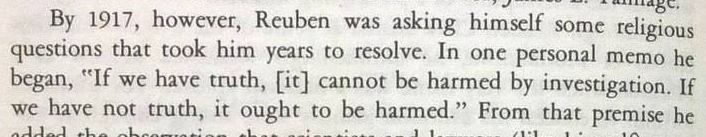
\includegraphics[width=0.4\linewidth]{articles/images/harm.png}
  \caption{J. Reuben Clark: The Church Years}
  \label{fig:clarkTruth}
\end{figure}

The quote should be cited in its full context of course. Because any and all 
sources should be found within their full context. Not only a portion. 
(See Appendix B: J. Reuben Clark: The Church Years)

Then there are the words of James E. Talmage:

\begin{displayquote}
The man who cannot listen to an argument which opposes his views either has a 
weak position or is a weak defender of it. No opinion that cannot stand 
discussion or criticism is worth holding. And it has been wisely said that the 
man who knows only half of any question is worse off than the man who knows 
nothing of it. He is not only one sided, but his partisanship soon turns him 
into an intolerant and a fanatic. In general it is true that nothing which 
cannot stand up under discussion and criticism is worth 
defending.\footnote{Editorial quoted in James E. Talmage, 
``Christianity Falsely So-Called," Improvement Era, Jan. 1920, 204.}
\end{displayquote}

George Albert Smith spoke on this very topic:

\begin{displayquote}
If a faith will not bear to be investigated; if its preachers and professors 
are afraid to have it examined, their foundation must be very 
weak.\footnote{George Albert Smith, Journal Of Discourses, v 14, page 216}
\end{displayquote}

Then M. Russell Ballard said the following counter claim:

\begin{displayquote}
We don't have to question anything in the church, don't get off into that. Just
stay in the Book of Mormon. Just stay in the Doctrine and Covenants. Just listen
to the prophets. Just listen to the apostles. We won't lead you astray, we
cannot lead you astray.\footnote{YSA Devotional, M. Russell Ballard, 2015}
\end{displayquote}

The church has released a handful of what they call Gospel Topic 
Essays.\footnote{https://www.lds.org/topics/essays?lang=eng} They are to shed
light on some of the history of the church that may or may not have been
widely known. This is a step in the right direction, however...it still feels
like the church is changing the narrative. Their history stated to the believers
has not always been the same. It has changed over time.

It is tempting to go through each of the essays...however I'm not sure I would
have the patience to go paragraph by paragraph and make notes on things found
and then look into the footnotes of each thing found.

Someday in the future I'm sure I will. There's no reason not to. If we are to
learn from the best books as it were, then the truth in those essays shouldn't
be scary. They should be welcomed with open arms. Is that possible in this day
and age of the internet? We have at our fingertips the ability to quickly search
for anything and everything. It could be considered dangerous.

I suppose, one needs to ask what is truth? If the truth can set you 
free,\footnote{John 8:32} then where exactly does the truth lay? Why is it so
difficult to find the truth at times? If the truth has been from the beginning
of the world, from before the beginning of the world, then it should be as
consistant as possible. It should be the same yesterday, today, tomorrow. All
truth should be the same and change shouldn't be a term in that narrative.

Yet the search for truth must go on.
\chapter{Revelation}

We live in a time of continuous revelation as it were. When the church was
being organized and during the time Joseph Smith was the prophet of the church,
he continued to receive revelations. The Doctrine and Covenants of the church
is full of revelations.

After Joseph's death, there doesn't appear to be many revelations coming forth
from the church. Some point to the end of polygamy, or the end of the ban 
against the blacks. There are those also who say there were other reasons
to end those things.

From a publication by David Whitmer, we find the following quote:

\begin{displayquote}
Some revelations are of God: 
some revelations are of man: 
and some revelations are of the devil.\footnote{David Whitmer, 
An Address to All Believers in Christ, in EMD 5: 198.}
\end{displayquote}

This is in regards to the failiure of the church to sell the copyright in
Canada. (See Appendix \ref{chap:believers})

Ahem, say what now? Revelations coming from the devil? As revelation? What?

How is that possible? It's been said that the devil can show himself as an 
angel, but an entire revelation from the devil? Wow, what kind of hot water
must you be in to get one of those?

Either way? How does one know if the revelation is from man, God, or the devil?
In what ways are we supposed to actually fully know that these things are
true and to do as they direct, or if we are to set them aside for they are evil?

Makes things rather complicated right?

After Joseph Smith's death, there weren't many additions to the Doctrine and
Covenants. No new revelations added. The Official Declarations 1 and 2 don't
appear to be revelations as they do not say ``Thus saith the Lord" in them,
which was known to be had in other revelations throughout the book.

So what are they exactly?

There's a revelation by Joseph F. Smith which became section 138 of the D\&C,
but nothing since then. Why is that? If we are a church that believes in
continuous revelations, why is that book not being updated? Why are there
not more revelations coming and recorded?

Time has changed things. Are people not as revelatory since the times of
Joseph Smith, Jr. when he led the church? Do we have all we need and God doesn't
see fit to speak to us in this day and age?

You might be thinking I'm being rude. But these are honest questions. I'm not
bashing the prophets who have come since Joseph Smith, Jr. I am just not aware
of actual revelations which have come along the way is all.

\section{Temple Changes}

Now the temple is a very sacred part of the LDS faith. People don't talk about
it openly due to covenants they have made inside the temple. It is supposedly
restored from the time of Adam when he walked the earth. Some say Joseph Smith
crated the Endowment based off of Freemasonry. Whatever the case, there have
been changes to the temple ritiual over the years.

\subsection{Oath to Avenge Joseph Smith}

After the death of Joseph Smith, Brigham Young added a vengence oath to the
endowment. It was to avenge the death of the Prophet Joseph Smith. If the temple
ordinance was restored and hadn't changed. I doubt this was actually intended to
be part of it. I doubt Adam went around swearing to an oath to avenge the death
of a man who wouldn't be born for centuries to come.

\subsection{Adam God Doctrine}

For a time the Adam God Doctrine was taught at the veil. This was instituted by
Brigham Young. What is the Adam God Doctrine? Here it is in short. Adam is God.
No seriously. Here it is in the long form:

\begin{displayquote}
Now hear it, O inhabitants of the earth, Jew and Gentile, Saint and sinner! 
When our father Adam came into the garden of Eden, he came into it with a 
celestial body, and brought Eve, one of his wives, with him. He helped to 
make and organize this world. He is MICHAEL, the Archangel, the ANCIENT OF 
DAYS! about whom holy men have written and spoken – He is our FATHER and our 
GOD, and the only God with whom WE have to do. Every man upon the earth, 
professing Christians or non-professing, must hear it, and will know it 
sooner or later!\footnote{Prophet Brigham Young, Journal of Discourses, v. 1, 
p. 51}
\end{displayquote}

This was all taught in the temple for a time before it was pulled from the
ceremony. If the temple ceremony was restored, per the Prophet Joseph Smith, why
was the Adam God Doctrine not there to begin with? Why was it added later to the
temple ceremony at the veil? Then, if it was taught as doctrine and was true,
why was it removed?

\subsection{Penalties}

Up until 1990, there were Penalties in the temple. People would symbolically cut
their throats as a sign for what would come if they were to give away the sacred
ordinances of the temple. These were in there from the start, and were removed
as I said in 1990. Is God changing His mind about what is to be taught? Why were
these removed from the temple ordinance? If it's no longer in there, were the
people who took the blood oaths still under requirement to live by those oaths
that if they talk of the temple they will be required to take their own lives?

Again something else that has changed from what was restored. If it is restored
is it not perfect? If it wsa perfect, the doctrine that is, then why was it
removed?

Perhaps it too closely resembled Cain's oath with Satan?

\begin{displayquote}
And Satan said unto Cain: Swear unto me by thy throat, and if thou tell it thou 
shalt die; and swear thy brethren by their heads, and by the living God, that 
they tell it not; for if they tell it, they shall surely die; and this that thy 
father may not know it; and this day I will deliver thy brother Abel into thine 
hands.\footnote{Moses 5:29}
\end{displayquote}

Was it a type of secret combination? We're told to avoid such things.

It should be interesting to note the following quote:

\begin{displayquote}
The Prophet Joseph Smith taught, `Ordinances instituted in the heavens before 
the foundation of the world, in the priesthood, for the salvation of men, 
are not to be altered or changed.'\footnote{Ensign Magazine, August 2002, p 22}
\end{displayquote}

\subsection{Other Changes}

There are other changes to the temple ceremony. At one point there was a
preacher who was a follower of Satan. An entire choir that would sing christian
hymns etc.

\subsection{Thou Shalt Not}

An interesting change is when God placed Adam in the Garden of Eden, he gave a
commandment:

\begin{displayquote}
But of the tree of the knowledge of good and evil, thou shalt not eat of it: 
for in the day that thou eatest thereof thou shalt surely 
die.\footnote{Genesis 2:17}
\end{displayquote}

Eve was not found on the Earth at that time.

In the temple we see that Adam and Eve were together in the Garden of Eden when
God gave such a commandment.

So which is correct? This isn't just what happened in Genesis, but it also
happened in the Book of Moses as well. God commands Adam to not eat of the
fruit, He then creates Eve later after pulling a rib from Adam's side. It is
again the same timeline in the Book of Abraham. So there are three sources from
which it is put forth, yet the temple contradicts that timeline. Again, which
one is correct?

Don't believe me? Here are the scriptures to research:

\begin{displayquote}
Genesis 2:15 - 22

Moses 3:15 - 22

Abraham 5: 11 - 16
\end{displayquote}
\section{Nephi or Moroni}

Another interesting fact that came up in early church history was the account of
Joseph Smith speaking to the prophet Nephi. Yes, Nephi. He originally said it
was Nephi who had visited him, not the angel Moroni. We can find this in the
Joseph Smith Papers:

\begin{displayquote}
The room was exceedingly light but not so much so as immediately around his 
person When I first looked upon <​him​> it I was afraid; but the fear soon left 
me: calling me by name, <he> said. that he was a messenger. sent from the 
presence of God to me. and that his name was Nephi.\footnote{
http://www.josephsmithpapers.org/paper-summary/history-circa-1841-draft-draft-3/6
}
\end{displayquote}

This was even publisehd in the Pearl of Great Price. It was later changed to
Moroni having visited Joseph Smith in what is the most current version of the
Pearl of Great Price.

Why the change? Why did Joseph change who had visited him? Who was it? Was it
Nephi or Moroni? If they both visited him, it was at different times. But the
narrative was changed to reflect that it was Moroni...after first being Nephi.
The experience, that one night, was changed. Why?
\chapter{Second Anointing and Calling and Election Made Sure}

There are some doctrines of the church that are not spoken of. Some doctrines 
have been abandoned by the church, disavowed as prophets speaking as men. 
Other doctrines of the church are simply not spoken about.

On lds.org, there is one doctrine that is mentioned with a strict warning not to 
discuss or answer questions about it. That is the doctrine of the second 
anointing.

In Chapter 19 of Doctrines of the Gospel Teacher Manual, it has the following 
caution:

\begin{displayquote}
Caution: Exercise caution while discussing the doctrine of having our calling 
and election made sure. Avoid speculation. use only the sources given here and 
in the student manual. Do \textit{not} attempt in any way to discuss or answer 
questions about the second anointing.
\end{displayquote}

So, uh what’s that about? That’s the only place on the lds.org website where 
that specific doctrine is mentioned. Now we obviously know what it is, but not 
how it is performed. Knowing what and knowing how are two very different things. 
Now you can google all you wish to know about it, I’m sure it’s been talked 
about. There’s no way it’s been kept secret for as long as it’s been known to 
the people of the earth. It’s out there. You just have to look for it.

 Now, some problems with this. Why would the manual provide a caution to not 
 discuss the second anointing? The second anointing is to seal up someone into 
 heaven. They are basically promised eternal life no matter what. The only thing 
 which could prevent them from going to heaven is murder or denying the Holy 
 Ghost.
 
 The second anointing is given to elite leaders of the church. The ordinance is 
 performed by the washing the feet of the couple in the temple. The couple are 
 anointed on the head with oil, their calling and election is made sure. That 
 is, they are guaranteed a place in the highest level of the Celestial Kingdom. 
 After which, the couple goes to a different room in the temple where the wife 
 washes the husbands feet and then lays her hands on his head and gives him a 
 priesthood blessing as the spirit directs. This is in preparation of death and 
 resurrection.
 
 Okay so that brought about an interesting twist. This is having received the 
 more sure word of prophecy. That is, you’re going past judgement day. Your fate 
 has already been made whole. You are basically judged taking God out of the 
 equation.
 
 First off, only God can judge us. That’s what a final judgement is for isn’t 
 it? How can a prophet of God or a man as it were proclaim that you are free of 
 the blood and sin of such a generation? That you are made clean and a King and 
 Priest unto God? Being a equal to that of Jesus Christ Himself.
 
 Second, we’re told that women cannot hold the priesthood in the church. She 
 cannot perform blessings, ordinances etc. Here during the second anointing this 
 is not he case. Not only does she perform an ordinance but she also performs a 
 blessing, not just a blessing though. It’s a blessing as the spirit directs. 
 So it is approved of God.
 
 I suppose this second part shouldn’t be much of a shock to me. Women have been 
 performing ordinances in the temple for years to other women. So perhaps we’ve 
 just been lied to all this time? It’s definitely something to look into for 
 sure.
 
 Now the calling and election made sure doctrine is to have Christ personally 
 visit you, it is determined that you will serve Christ no matter the cost. He 
 gives unto you the second comforter, that is the visitation of Christ.
 
 According to the caution above, it appears the calling and election being made 
 sure and the second anointing are two separate ordinances. For one you actually 
 see Christ the other you are just given the ability to be a God basically.
 
 We read about the calling and election being made sure in 2 Peter 1:10.
 
 \begin{displayquote}
 Wherefore the rather, brethren, give diligence to make your calling and 
 election sure; for if ye do these things, ye shall never fail:
 \end{displayquote}
 
 In the experiences I’ve read regarding the second anointing. Why is it only the 
 man is anointed a King and Priest to the Most High God? The woman is not 
 anointed along with her husband. Why is that? She performs the ordinance on him 
 after the apostle performs the ordinance and gives her husband a blessing. But 
 the husband does not in return give her a blessing and does not wash her feet. 
 Perhaps there are times when the woman is also anointed a Queen and Priestess, 
 the website ldsendowment.org has instructions for the entire process including 
 having the wife anointed. So perhaps in just the experiences I’ve read it was 
 only the husband. You may also read about this in a book by David John Buerger 
 titled "The Mysteries of Godliness."

 This doctrine is not taught in the church. It has been made known to us by 
 people who have experienced it. They have since fallen away from the church 
 because they have come to the conclusion that it is not true. But they have 
 brought forth the knowledge they have gained in this life with them thus far, 
 and that is well enough.

 There is also a paper titled “The Fulness of the Priesthood: The Second 
 Anointing in Latter-day Saint Theology and Practice” by David John Buerger. 
 According to that paper the second anointing was rather common to be had among 
 the saints. Prophets authorized the second anointing in the low thousands. It 
 makes one stop to think for a moment, why did it cease? Or well, I suppose it 
 dropped in number, not ceased. I would wager it takes place still today just 
 not as much as it used to.
\section{Carthage Jail}

Joseph was arrested for civil disturbance. Well he went to answer charges
because of it. But he states the following:
\begin{displayquote}
I know not why; but for some reason I am constrained to hasten my  preparations, 
and to confer upon the Twelve all the ordinances, keys,  covenants, endowments, 
and sealing ordinances of the priesthood, and so  set before them a pattern in 
all things pertaining to the sanctuary and  the endowment therein. (Quoted by 
Parley P. Pratt in "Proclamation to  The Church of Jesus Christ of Latter-day 
Saints," Millennial Star, Mar. 1845, 151.)\footnote{
https://history.lds.org/article/historic-sites/illinois/carthage/carthage-jail?lang=eng
}
\end{displayquote}

If he wouldn't have passed on those keys etc to the 12, they wouldn't still be 
around. Would he have died at Carthage or would he have escaped that situation? 
Because God wouldn't have a 2nd "apostasy", would he?
\chapter{Literal vs Symbolic}

The LDS Church is full of symbolism, the temple being one of the biggest symbols of
all. However the bible contains stories which can be considered literal, or symbolic
as well. A few to mention are Noah and the great flood, and Jonah swalled by the
whale (although I think the bible actually says it's a big fish).

So which is it? Are these stories factual? Are they symbolic in nature to be faith
promoting stories? What of the Book of Mormon, is it factual? Is it faith promoting?

There are creatures talked about in the bible which we consider mystical today. But
according to the Bible Dictionary, they are more of an ox. Yes, I'm talking about the
Unicorn.

Unicorns? Unicorns.

Here are the places in the bible where it mentions these creatures:

\begin{displayquote}
He maketh them also to skip like a calf; Lebanon and Sirion like a young 
unicorn.\footnote{Psalms 29:6}
\end{displayquote}

\begin{displayquote}
Will the unicorn be willing to serve thee, or abide by thy crib?\footnote{Job 39:9}
\end{displayquote}

\begin{displayquote}
Canst thou bind the unicorn with his band in the furrow? or will he harrow the 
valleys after thee?\footnote{Job 39:10} 
\end{displayquote}

\begin{displayquote}
God brought them out of Egypt; he hath as it were the strength of an 
unicorn.\footnote{Numbers 23:22}
\end{displayquote}

\begin{displayquote}
But my horn shalt thou exalt like the horn of an unicorn: I shall be 
anointed with fresh oil.\footnote{Psalms 92:10}
\end{displayquote}

\begin{displayquote}
God brought him forth out of Egypt; he hath as it were the strength of an 
unicorn: he shall eat up the nations his enemies, and shall break their 
bones, and pierce them through with his arrows.\footnote{Numbers 24:8}
\end{displayquote}

\begin{displayquote}
And the unicorns shall come down with them, and the bullocks with the bulls; and 
their land shall be soaked with blood, and their dust made fat with 
fatness.\footnote{Isaiah 34:7} 
\end{displayquote}

\begin{displayquote}
Save me from the lion’s mouth: for thou hast heard me from the 
horns of the unicorns.\footnote{Psalms 22:21}
\end{displayquote}

\begin{displayquote}
His glory is like the firstling of his bullock, and his horns are like the horns 
of unicorns: with them he shall push the people together to the ends of the 
earth: and they are the ten thousands of Ephraim, and they are the thousands 
of Manasseh.\footnote{Deuteronomy 33:17} 
\end{displayquote}

And then of course we have the Bible Dictionary description:

\begin{displayquote}
A wild ox, the \textit{Bos primigenius}, now extinct, but once common in Syria. 
The KJV rendering is unfortunate, as the animal intended is two-horned.\footnote{
LDS Bible Dictionary: Unicorn
}
\end{displayquote}

Scholars have indicated that it is not the actual mystical creature unicorn which we
have come to know and love. Which is kind of a disappointment. But if it can be in
there, and be misinterpreted in these days, what else might the bible be hiding?
\chapter{Polygamy and Polyandry}

First off, let's get some definitions out of the way:

\begin{displayquote}
Polygamy: The practice or custom of having more than one wife or husband at the same 
time.
\end{displayquote}

\begin{displayquote}
Polyandry: Polygamy in which a woman has more than one husband.
\end{displayquote}

Eveyone knew Brigham Young practiced polygamy. It was thought for the longest time 
that it all began with him. Well, that's not the case. According to the LDS Church
Essay, ``Plural Marriage in Kirtland and Nauvoo"\footnote{
https://www.lds.org/topics/plural-marriage-in-kirtland-and-nauvoo?lang=eng
} we learn that Joseph Smith practed polygamy.

From the book of Jacob, we read:

\begin{displayquote}
For if I will, saith the Lord of Hosts, raise up seed unto me, 
I will command my people; otherwise they shall hearken unto these 
things.\footnote{Jacob 21:30}
\end{displayquote}

Polygamy is meant to bring up seed unto the Lord. It's a means of populating the
Earth so those people will become members of the Lord's church and continue on with
the traditions of their fathers.\footnote{Not to be confused with the vain traditions
of the wicked Lamenites.}

If that's ``one" of the reasons for practicing polygamy, why are there no offspring
of Joseph Smith from those polygmous relationships? People in the church will tell
you he married them spiritually only, but that goes against what the Book of Mormon
teaches.

Can't have it both ways, so which is it?

There are also reports of Joseph Smith marrying girls as young as 15.\footnote{
From the essay: ``The youngest was Helen Mar Kimball, daughter of Joseph’s close 
friends Heber C. and Vilate Murray Kimball, who was sealed to Joseph several 
months before her 15th birthday."
} Again, the apologetics will tell you this was normal for the time. Normal or not,
it goes against any kind of morality a person should have. I don't care the time
period in which it was normal.

Joseph was also sealed to women who were already married to other men. According to
the essay, an angel rebuked Joseph for practicing Polyandry and went back to marrying
single women.

Another moment where God forgot to specifcially announce His intentions of how
polygamy should be practiced? Again, one would think that God would have instructed
Joseph exactly in how things should be worked out. The Bible is full of examples
of the Lord telling the people exactly how to build something, why would other
principles of the gospel be any different?

Is it possible, the polygamy command didn't come from God at all? Joseph made it up
and he decided what he wanted to do and how to go about it? If that's the case,
that's not how God is meant to work. One would hope that certain commandments given
from God would have a strict understanding and expectation to be followed. A prophet
is speaking for God afterall, is he not?

Again from the same essay ``Plural Marriage in Kirtland and Nauvoo" stated above,
there is a troubling line:

\begin{displayquote}
But Emma likely did not know about all of Joseph’s sealings.
\end{displayquote}

This goes against D\&C 132.\footnote{
D\&C 132:52 And let mine handmaid, Emma Smith, receive all those that have been 
given unto my servant Joseph, and who are virtuous and pure before me; and those 
who are not pure, and have said they were pure, shall be destroyed, saith the 
Lord God.
} She was to receive all those who the Lord gave unto Joseph. if she did not know
about them, how was she to receive them? Apparently this revelation was directed
directly to Emma because she did not apporve of Joseph's polygamy practices.

There is another clause in there, if she doesn't accept Joseph's other wives, he is
exempt from the Law of Sarah and can marry other wives anyway. So even if Emma didn't
want to accept it, Joseph could go ahead and marry others as he saw fit.\footnote{
D\&C 132:65 Therefore, it shall be lawful in me, if she receive not this law, for him
to receive all things whatsoever I, the Lord his God, will give unto him, because she
did not believe and administer unto him according to my word; and she then becomes
the transgressor; and he is exempt from the law of Sarah, who administered unto
Abraham according to the law when I commanded Abraham to take Hagar to wife.
}

Polygamy came to an end in 1890 with the manifesto. Official Declaration 1 in the
LDS Scriptures. Well kinda. They had to put out a second manifesto in 1904 warning
people they would be excommunicated if they entered into plural marriage. So I guess
the first one was to say the church didn't believe in the practice, and the second
was to actually enforce the rule? I'm not quite sure.\footnote{
``The Manifesto and the End of Plural Marriage"
https://www.lds.org/topics/the-manifesto-and-the-end-of-plural-marriage?lang=eng
}

There were mixed feelings on the first manifesto to begin with, I've no idea how
people felt about the second manifesto. Not much is talked about the second manifesto
in today's church meetings. Only the first. There's a bit of things people aren't
taught about in the church, a lot of history gets glossed over; this is one of them.

In the 1835 Book of Commandments, there is an article titled Marriage. In this
article it is stated that the church only believed in monogomy. There is a little
history behind this. It is claimed by Joseph Fielding Smith that Oliver Cowdery
inserted the document ``without authority". That is to say words were put into the
1835 D\&C and the Prophet Joseph Smith did nothing to stop it.

On July 7, 1878, Joseph F. Smith talked about Oliver's writing of this article:

\begin{displayquote}
To put this matter more correctly before you, I here declare that the principle of 
plural marriage was not first revealed on the 12th day of July, 1843. It was 
written for the first time on that date, but it had been revealed to the Prophet 
many years before that, perhaps as early as 1832. About this time, or 
subsequently, Joseph, the Prophet, intrusted this fact to Oliver Cowdery; he 
abused the confidence imposed in him, and brought reproach upon himself, and 
thereby upon the church by ``running before he was sent," and "taking liberties 
without license," so to speak, hence the publication, by O. Cowdery, about this 
time, of an article on marriage, which was carefully worded, and afterwards found 
its way into the Doctrine and Covenants without authority. This article explains 
itself to those who understand the facts, and is an indisputable evidence of the 
early existence of the knowledge of the principle of patriarchal marriage by the 
Prophet Joseph, and also by Oliver Cowdery.\footnote{Joseph F. Smith, Journal of 
Discourses 20:29.}
\end{displayquote}

How is this possible that something made it into the Doctrine and Covenants without
Joesph's knowledge? It wasn't given as a revelation, it was something Oliver wrote up
himself. If that's the case? What other writings in the Doctrine and Covenants are
just the thoughts of man and not revelations?

Was Joseph Smith trying to hide polygamy from the followers of the church? It's known
that polygamy wasn't widely practiced. Considering his own wife, Emma, signed her
name on an article saying that polygamy is not practiced. She didn't know he was
marrying other women at the time or, did she know and she was lying about it?

Figure \ref{fig:tas1} shows her name and what she signed.

\begin{figure}[h!]
  \centering
  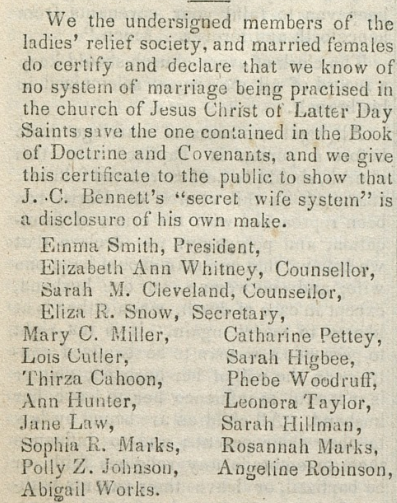
\includegraphics[width=0.4\linewidth]{articles/images/polygamy.png}
  \caption{Times and Seasons Vol 3 No. 23}
  \label{fig:tas1}
\end{figure}

The quesiton arises, at which point in time did Emma learn of plural marriage? 
Joseph began practicing plural marriage possibly as early as 1832, as mentioned by
Joseph Fielding Smith above, so it was in practice at the time Oliver published the
article in the D\&C.

Another interesting aspect of D\&C Section 132 regarding the apporval of polygamy:

\begin{displayquote}
David also received many wives and concubines, and also Solomon and Moses my 
servants, as also many others of my servants, from the beginning of creation until 
this time; and in nothing did they sin save in those things which they received 
not of me.

David’s wives and concubines were given unto him of me, by the hand of Nathan, 
my servant, and others of the prophets who had the keys of this power; and in none of 
these things did he sin against me save in the case of Uriah and his wife; and, 
therefore he hath fallen from his exaltation, and received his portion; and he 
shall not inherit them out of the world, for I gave them unto another, saith the 
Lord.\footnote{D\%C 132:38-39}
\end{displayquote}

Okay, so David had many wives and those were given to him of the Lord. So he was
commanded to have multiple wives. Yet, there is a footnote in verse 39, which points
over to the Book of Mormon:

\begin{displayquote}
But the word of God burdens me because of your grosser crimes. For behold, 
thus saith the Lord: This people begin to wax in iniquity; they understand not the 
scriptures, for they seek to excuse themselves in committing whoredoms, because of 
the things which were written concerning David, and Solomon his son.

Behold, David and Solomon truly had many wives and concubines, which thing was 
abominable before me, saith the Lord.\footnote{Jacob 2:23-24}
\end{displayquote}

Now we're learning that David's wives were an abomination before the Lord. They were
not commanded of Him. But in D\&C it says the Lord gave them to him. So, which is it
exactly? Why is there a contradiction to it all?
\section{Doctrine of Christ}

We are told in the Book of Mormon that the Doctrine of Christ is fourfold:

\begin{enumerate}
  \item Faith
  \item Repentance
  \item Baptism
  \item Receive the Holy Ghost
\end{enumerate}

This is found in 2nd Nephi 31-32, there it states the Doctrine of Christ and the
results of receiving the Doctrine of Christ. Covenants with established blessings
attached to them.

The Book of Mormon then reiterates it in 3rd Nephi chapter 11. Again it establishes
Christ's Doctrine. We are to be baptized in Christ's name. But near the end of the
chapter, it says that ``whoso shall declare more or less than this, and establish it
for my doctrine, the same cometh of evil, and is not built upon my rock."\footnote{
3 Nephi 11:40
} It goes on to say how the person will be thrust down to hell etc.

The Church of Jesus Christ of Latter-day saints declares its doctrine to be more than
that which Christ has spoken, how does the church get around it? What are their
explainations for adding to the doctrine of Jesus Christ?

I find it troubling the churche's own scripture even says not to add to it, and yet
they have. I suppose one could argue the church isn't adding to the Doctrine of
Christ, but adding to the doctrine as a whole. The doctrine of Christ remains
untouched. But is not Christ the church and that doctrine would be the same?

To me, these scriptures teach that we are to repent of our sins, be baptized and
become like a little child. We are then able to inherit the kingdom of God. It
doesn't say anything about having to go to the temple, pay tithing etc. Those things
are not requirements to be with God. Yet the church claims those are requirements,
that one cannot dwell with God without having all of those necessary ordinances done.

Are not those other ordinances additions to the Doctrine of Christ? The same thing
which Jesus had warned against having additions to?

According to ``Teaching in the Savior's way" there are nine doctrinal principles the
church has. They are:

\begin{enumerate}
  \item Godhead
  \item Plan of Salvation
  \item Atonement of Jesus Christ
  \item Dispensation, Apostasy, and Restoration
  \item Prophets and Revelation
  \item Priesthood and Priesthood Keys
  \item Ordinances and Covenants
  \item Marriage and Family
  \item Commandments
\end{enumerate}

Is this not adding to Christ's Doctrine, that which is required to get into heaven?
If Christ's Doctrine is easy and simple to understand so everyone can take part and
if they try hard enough, they can come back to God. Which is what God want's right? I
can't see a God forcing His children to jump through hoops in order to get back to
His presence. Well, the church would tell you they aren't forcing anyone to jump
through hoops, if they don't want to play by the rules they'll be excommunicated.

If a man professes Christ to be their Lord and Savior, repents of their sins gets 
baptized and receives the Holy Ghost; why can't they be saved? Why does there need to
be additional doctrines and teachings out there?

Some will claim it goes back to authority. Who gave Adam authority to baptize? Why is
there no record of Adam baptizing Eve in the Bible? Wouldn't that be one of the
truths transcribers would leave in there if it's so important?

Oh, according to the Joseph Smith Translatin of the bible, chapter 6 of Genesis
states:

\begin{displayquote}
64 And it came to pass, when the Lord had spoken with Adam, our father, that Adam 
cried unto the Lord, and he was caught away by the Spirit of the Lord, and was 
carried down into the water, and was laid under the water, and was brought forth 
out of the water.

65 And thus he was baptized, and the Spirit of God descended upon him, and thus he 
was born of the Spirit, and became quickened in the inner man.

66 And he heard a voice out of heaven, saying: Thou art baptized with fire, and with 
the Holy Ghost. This is the record of the Father, and the Son, 
from henceforth and forever;\footnote{JST Genesis 6:64-66}
\end{displayquote}

Well that brings about an interesting question. The Holy Ghost baptized Adam, and
then descended upon him? Without someone laying hands on Adam to give him the gift of
the Holy Ghost? So it's not even the same way the LDS Church teaches it to be? Surely
God would have set the correct course for baptism with Adam, wouldn't He have?

There is of course the conflicting account where Alma baptizes himself:

\begin{displayquote}
12 And now it came to pass that Alma took Helam, he being one of the first, and went 
and stood forth in the water, and cried, saying: O Lord, pour out thy Spirit upon thy 
servant, that he may do this work with holiness of heart.

13 And when he had said these words, the Spirit of the Lord was upon him, and he 
said: Helam, I baptize thee, having authority from the Almighty God, as a testimony 
that ye have entered into a covenant to serve him until you are dead as to the mortal 
body; and may the Spirit of the Lord be poured out upon you; and may he grant unto 
you eternal life, through the redemption of Christ, whom he has prepared from the 
foundation of the world.

14 And after Alma had said these words, both Alma and Helam were buried in the 
water; and they arose and came forth out of the water rejoicing, being filled with 
the Spirit.

15 And again, Alma took another, and went forth a second time into the water, and 
baptized him according to the first, only he did not bury himself again in the 
water.\footnote{Mosiah 18:12-15}
\end{displayquote}

Why didn't the Holy Ghost baptize Alma like he did Adam? Where did Alma get the
authority to baptize \textit{before} being baptized himself?
\chapter{Seeing God or Jesus}

Is it possible that since the early days of the Church in the old world, that no man
has seen God or Jesus?

Think about it for a moment. In times past, when God wanted to communicate His word
to people He sent angels to talk with them. He didn't make an appearance Himself.

We know in the Garden of Eden, God appeared to Adam and Eve. But afterwards when He
sent further light and knowledge to them, it was done through His people. God didn't
appear to them.

The God of the Old Testament didn't appear to Moses face to face, but through a
burning bush.

So why was it necessary for God to appear to Joseph Smith when an angel could have
done exactly that. Doesn't God believe in sending messengers down to people? Isn't
that his modus operandi?

Even then, it was a vision. Did Joseph see it in his minds eye? And why did Satan
attempt to stop him from praying? If Satan truly doesn't know the mind of God, why
would he stop a fourteen year old boy from praying to God? Did Satan actually know
God and Jesus were about to visit? If so, then Satan knows somewhat the mind of God
does he not?

We know there are some instances in the New Testament where people have seen Jesus.
They weren't the most righteous people of their time, Saul was out persecuting the
church, yet he saw Jesus or heard Jesus, it depends on which account you read. Here
was by all accounts an evil man who was out trying to destroy the church of God and
Jesus made himself known unto this man.

Propehts and apostles in these latter days, aside from Joseph Smith, do not declare
to have seen God and Jesus. It isn't done anymore. Why is that? If they're God's
mouthpiece, wouldn't they be in contact with God and Jesus? Some say, yes but they
receive revelation. Is that enough? Wouldn't they at least need to have that personal
touch like Joseph Smith did?
\chapter{The Prophet}

It has been said, when the prophet speaks the debate is over.\footnote{
Ensign, Nov. 1978, p. 108
}

That when ``our leaders speak, the thinkikng has been done."\footnote{Improvement 
Era, June 1945}

Ezra Taft Benson, then a member of the Quorum of the Twelve Apostles, said the
following:

\begin{displayquote}
The prophet does not have to say ``Thus saith the Lord" to give us
scripture.\footnote{Fourteen Fundamentals in Following The Prophet, Ezra Taft 
Benson, 1980}
\end{displayquote}

He then went on to Quote Brigham Young, who said:

\begin{displayquote}
I have never yet preached a sermon and sent it out to the children of men, that 
they may not call scripture.\footnote{Journal of Discourses, 13:95.}
\end{displayquote}

I wonder if Benson even read some of the things Brigham had taught over the years?
He's quoting from the Journal of Discourses, so he should have some knowledge of
things that Brigham actually taught as doctrine. One would think this would be the
case.

To be taught to always follow the prophet no matter what, it's blind obedience.
There's no other way of saying what it is. That's exactly what it is. When a group is
told to not think about it, to simply follow a living prophet and what he says goes?
It feels much like being led down a path where you have no say in anything. If a
person even thinks about disagreeing with that prophet? They are in danger of being
called an apostate.

Here is the full list of what Ezra Taft Benson stated in his talk.

\begin{displayquote}
\begin{enumerate}
\item The prophet is the only man who speaks for the Lord in everything.
\item The living prophet is more vital to us than the standard works.
\item The living prophet is more important to us than a dead prophet.
\item The prophet will never lead the church astray.
\item The prophet is not required to have any particular earthly training or 
credentials to speak on any subject or act on any matter at any time.
\item The prophet does not have to say ``Thus saith the Lord," to give us scripture.
\item The prophet tells us what we need to know, not always what we want to know.
\item The prophet is not limited by men's reasoning.
\item The prophet can receive revelation on any matter, temporal or spiritual.
\item The prophet may advise on civic matters.
\item The two groups who have the greatest difficulty in following the prophet are 
the proud who are learned and the proud who are rich.
\item The prophet will not necessarily be popular with the world or the worldly.
\item The prophet and his counselors make up the First Presidency-the highest 
quorum in the Church.
\item The prophet and the presidency-the living prophet and the First 
Presidency-follow them and be blessed-reject them and suffer.\footnote{Fourteen 
Fundamentals in Following The Prophet, Ezra Taft Benson, 1980}
\end{enumerate}
\end{displayquote}

Though the prophet at the time, President Kimball, and the Quorum of the Twelve
Apostles did not agree with the words of Benson, because they set the prophet up as
being perfect, a man who could not fail. The talk was never changed and was never
retracted.

In later years, we are told that prophets are not always speaking as a prophet.
Sometimes they are speaking as a man. It becomes difficult to understand when a
prophet is talking for God and when he is talking as a man. Conflicting thoughts and
speaches, quotes abound, some of which have been discussed already.

Let's take a look at some quotes where the prophet spoke, shall we? I'll let you
decide if they were speaking as a man or from God.

\begin{displayquote}
The attitude of the Church with reference to Negroes remains as it has always 
stood. It is not a matter of the declaration of a policy but of direct commandment 
from the Lord, on which is founded the doctrine of the Church from the days of 
its organization, to the effect that Negroes may become members of the Church 
but that they are not entitled to the priesthood at the present time.\footnote{
The First Presidency on the Negro Question, 17 Aug. 1949.
}
\end{displayquote}

\begin{displayquote}
Shall I tell you the law of God in regard to the African race? If the white man 
who belongs to the chosen seed mixes his blood with the seed of Cain, the penalty, 
under the law of God, is death on the spot. This will always be so. The nations of 
the earth have transgressed every law that God has given, they have changed the 
ordinances and broken every covenant made with the fathers, and they are like a 
hungry man that dreameth that he eateth, and he awaketh and behold he is
empty.\footnote{Prophet Brigham Young, Journal of Discourses, v. 10, p. 110}
\end{displayquote}

\begin{displayquote}
I [am] opposed to hanging, even if a man kill another, I will shoot him, or cut 
off his head, spill his blood on the ground, and let the smoke thereof ascend up t
o God; and if ever I have the privilege of making a law on that subject, 
I will have it so.\footnote{Prophet Joseph Smith, Jr., History of the Church, v. 
5, p. 296, 1949}
\end{displayquote}

\begin{displayquote}
Will you love your brothers and sisters likewise, when they have committed a sin 
that cannot be atoned for without the shedding of their blood? Will you love that 
man or woman well enough to shed their blood? That is what Jesus Christ
meant.\footnote{Prophet Brigham Young, Deseret News, April 16, 1856}
\end{displayquote}

\begin{displayquote}
Suppose you found your brother in bed with your wife, and put a javelin through 
both of them. You would be justified, and they would atone for their sins, and be 
received into the Kingdom of God. I would at once do so, in such a case; and under 
the circumstances, I have no wife whom I love so well that I would not put a 
javelin through her heart, and I would do it with clean hands.... There is not a 
man or woman, who violates the covenants made with their God, that will not be 
required to pay the debt. The blood of Christ will never wipe that out, your own 
blood must atone for it.\footnote{Prophet Brigham Young, Journal of Discourses, v. 
1, pp. 108-109}
\end{displayquote}

\begin{displayquote}
Joseph Smith taught that there were certain sins so grievous that man may commit, 
that they will place the transgressors beyond the power of the atonement of Christ. 
If these offenses are committed, then the blood of Christ will not cleanse them 
from their sins even though they repent. Therefore their only hope is to have 
their blood shed to atone, as far as possible, in their behalf. This is scriptural 
doctrine, and is taught in all the standard works of the Church.\footnote{
Prophet Joseph Fielding Smith, Doctrines of Salvation, v. 1, pp. 135-136, 1954
}
\end{displayquote}

There are some interesting ``doctrine" taught here. (They claim it's doctrine so
is it not?) Were these men teaching as prophets or their own thoughts? They claim
it's doctrine, and that's how things are. So what is a person to believe regarding
it?

\section{Speaking as a Man}

In early 1961, Joseph Fielding Smith preached to a stake conference congregation in 
Hawaii:

\begin{displayquote}
We will never get a man into space. This earth is man's sphere and it was never 
intended that he should get away from it. The moon is a superior planet to the 
earth and it was never intended that man should go there. You can write it down in 
your books that this will never happen.\footnote{D. Michael Quinn, Elder statesman: 
A Biography of J. Reuben Clark (Salt Lake City, Utah: Signature Books, 2002) p. 498.}

Earlier, Smith had written that ``it is doubtful that man will ever be permitted 
to make any instrument or ship to travel through space and visit the moon or any 
distant planet".\footnote{Joseph Fielding Smith, Answers to Gospel Questions (Salt 
Lake City, Utah: Deseret Book, 1957) 2:191.} At the 1970 press conference where Smith 
was introduced as President of the LDS Church, he was asked about these statements; 
Smith reportedly responded, ``Well, I was wrong, wasn't I?"\footnote{
Adam Kotter, ``When Doubts and Questions Arise", Liahona, March 2015.
}
\end{displayquote}

At least a prophet had the ability to state he was wrong. You don't see that happen
much these days. To admit to being wrong shows a lack of strength and signs of
weakness.

This was not the first time a prophet has spoken about space.

\begin{displayquote}
`` `Inhabitants of the Moon are more of a uniform size than the inhabitants of the 
Earth, being about 6 feet in height. They dress very much like the Quaker Style \& 
are quite general in Style, or the one fashion of dress. They live to be very old; 
comeing [sic] generally, near a thousand years.' This is the description of them as 
given by Joseph the Seer, and he could `See' whatever he asked the Father in the 
name of Jesus to see."\footnote{
Prophet Joseph Smith, Jr., in Journal of O.B. Huntington, Book 14, p. 166
}
\end{displayquote}

\begin{displayquote}
``Who can tell us of the inhabitants of this little planet that shines of an evening,
called the moon?... When you inquire about the inhabitants of that sphere you find 
that the most learned are as ignorant in regard to them as the ignorant of their 
fellows. So it is in regard to the inhabitants of the sun. Do you think it is 
inhabited? I rather think it is. Do you think there is any life there? No question 
of it; it was not made in vain."\footnote{
Prophet Brigham Young, Journal of Discourses, v. 13, p. 271
}
\end{displayquote}

\begin{displayquote}
``If [the sun] was made to give light to those who dwell upon it, and to other
planets; and so will this earth when it is celestialized. Every planet in the first 
rude, organic state receives not the glory of God upon it, but is opaque; but when 
celstialized, every planet that God brings into existence is a body of light, but 
not till then."\footnote{
Prophet Brigham Young, Journal of Discourses, v. 13, p. 271
}
\end{displayquote}

\section{The Living Prophet is more important than the scriptures.}

It has been said that basically the current or modern prophet is more important than
the scriptures. The exact words were: 
``The living prophet is more vital to us than the Standard Works."\footnote{Fourteen 
Fundamentals in Following the Prophet, Ezra Taft Benson, June 1981, LDS.org}

\begin{displayquote}
We are admonished to ``seek out of the best books words of wisdom" (D\&C 88:118). 
Surely these books must include the scriptures. Alongside them must be the words of 
the Presidents of the Church. The Lord said of the President of the Church, ``His 
word ye shall receive, as if from mine own mouth" (D\&C 21:5). These books make up 
what has been referred to as ``the Lord’s library"—namely the standard works and 
the various volumes that contain the words of the different Presidents of the Church. 
Of the latter volumes, that which would be of greatest importance to you would be 
the words of the current President of the Church, for his words are directed to our 
day and our needs. (Teachings of Ezra Taft Benson, p.137-138)
\end{displayquote}

\begin{displayquote}
I will refer to a certain meeting I attended in the town of Kirtland in my early 
days. At that meeting some remarks were made that have been made here today, with 
regard to the living oracles and with regard to the written word of God. The same 
principle was presented, although not as extensively as it has been here, when a 
leading man in the Church got up and talked upon the subject, and said: 
``You have got the word of God before you here in the Bible, Book of Mormon, and 
Doctrine and Covenants; you have the written word of God, and you who give 
revelations should give revelations according to those books, as what is written in 
those books is the word of God. We should confine ourselves to them." When he 
concluded, Brother Joseph turned to Brother Brigham Young and said, ``Brother 
Brigham I want you to take the stand and tell us your views with regard to the 
written oracles and the written word of God." Brother Brigham took the stand, and 
he took the Bible, and laid it down; he took the Book of Mormon, and laid it down; 
and he took the Book of Doctrine and Covenants, and laid it down before him, and he 
said: ``There is the written word of God to us, concerning the work of God from the 
beginning of the world, almost, to our day." ``And now," said he, ``when compared 
with the living oracles those books are nothing to me; those books do not convey 
the word of God direct to us now, as do the words of a Prophet or a man bearing the 
Holy Priesthood in our day and generation. I would rather have the living oracles 
than all the [p.23]writing in the books." That was the course he pursued. When he was 
through, Brother Joseph said to the congregation: ``Brother Brigham has told you the
word of the Lord, and he has told you the truth."  (Conference Report, 
  October 1897, p.22)
\end{displayquote}

\section{I am so sustained}

On two events, many many years apart, two prophets have said ``I am so sustained"
when asked if they were a prophet, seer, and revelator.

The first was from Joseph F. Smith:

\begin{displayquote}
Mr. Tayler. Are you propeht, seer, and revelator?

Mr. Smith. I am so sustained and upheld by my people.\footnote{Reed Smoot Hearings}
\end{displayquote}

The second, was during an interview with Gordon B. Hinckley:

\begin{displayquote}
Q: You are the president, prophet, seer and revelator of the Mormon Church?

A: I am so sustained, yes. (Laughter)\footnote{SUNDAY INTERVIEW -- Musings of the 
Main Mormon / Gordon B. Hinckley, `president, prophet, seer and revelator' of the 
Church of Jesus Christ of Latter-day Saints, sits at the top of one of the world's 
fastest-growing religions (sfgate.com) }
\end{displayquote}

In that second quote, I wonder why there was laughter? Would not the prophet of the
church take it with all seriousness? Was it a nervous laugh? What exactly was it?

I find the same phrased used to be interesting as well. Did Hinckley simply know of
the Reed Smoot hearings before he answered the question and gave the same response?
Are they told to give that response? Was it just coincidence?

\section{Follow The Prophet}

As a primary child, we sang ``Follow the Prophet". If we follow the prophet we won't
go astray, at least that is the thought behind the song; which repeats over and over
again.

The apostle Marion G. Romney had the following to say regarding the prophet, well the
president of the church.

\begin{displayquote}
I was greatly impressed by the President's remarks. I am glad he said what he did. 
Listening to him, I was taken back in my thoughts a quarter of a century to an 
experience I had with President Heber J. Grant. We were discussing some criticism 
that had been directed against an action taken by him in his official capacity. 
Putting his arm across my back and resting his hand on my left shoulder, he said, 
``My boy, you always keep your eye on the President of the Church, and if he tells 
you to do something wrong, and you do it, the Lord will bless you for it."

And then he added, ``You don't need to worry, however; the Lord will never let his
mouthpiece lead his people astray."\footnote{Apostle Marion G. Romney, 
``The Covenant of the Priesthood," Ensign, July 1972, p. 98}
\end{displayquote}
\chapter{The Apostles}

According to the Encylopedia of Mormonism:

\begin{displayquote}
An `apostle' is an ordained leader in the Melchizedek Priesthood in The Church of 
Jesus Christ of Latter-day Saints. Apostles are chosen through inspiration by the 
President of the Church, sustained by the general membership of the Church, and 
ordained by the First Presidency and Quorum of the Twelve Apostles by the laying 
on of hands. They serve as general authorities-as distinguished from local and 
regional officers-holding their office as apostle for the duration of their lives. 
The senior apostle is the President of the Church. In addition to serving as 
witnesses of Jesus Christ to all the world (D\&C 107:23), as Jesus' apostles did, 
members of the current Quorum of the Twelve Apostles hold the keys of the 
priesthood—that is, the rights of presidency (D\&C 107:35; cf. 
124:128)\footnote{Encyclopedia of Mormonism [1992], 1:59–60}
\end{displayquote}

In Jesus' time, the apostles were actual witnesses of Christ. That is, they saw Him
and could testify of seeing Him. The apostles in these latter-days, don't appear to
have had that blessing of seeing the Savior. They are a witness of Him in name only.

During a youth event in WA, Elder Oaks at the time responded to the following
question:

\begin{displayquote}
\textbf{Youth Asks:}

\textit{What should we pray for to receive the same testimony and/or conversion that 
Alma the Younger experienced, for our friend who are not members?}

\textbf{Elder Oaks answers:}

I've never had an experience like that and I don't know anyone among the 1st 
Presidency or Quorum of the 12 who've had that kind of experience. Yet everyone of 
us knows of a certainty the things that Alma knew. But it's just that unless the Lord 
chooses to do it another way, as he sometimes does; for millions and millions of His 
children the testimony settles upon us gradually. Like so much dust on the windowsill 
or so much dew on the grass. One day you didn't have it and another day you did and 
you don't know which day it happened. That's the way I got my testimony. And then I 
knew it was true when it continued to grow.\footnote{Multi-Stake Youth Fireside 
Bellevue, WA, 1/23/2016}
\end{displayquote}

Some say that is talking only about an Alma the Younger experience, even though Oaks
says he didn't have a miraculous experience, that his testimony grew over time.

Okay, how about the Prophet Joseph Fielding Smith?

\begin{displayquote}
The question frequently arises: ``Is it necessary for a member of the Council of the
Twelve to see the Savior in order to be an apostle?" It is their privilege to see him
if occasion requires, but the Lord has taught that there is a stronger witness than
seeing a personage, even of seeing the Son of God in a vision. Impressions on the
soul that come from the Holy Ghost are far more significant than a vision. When
Spirit speaks to spirit, the imprint upon the soul is far more difficult to erase.
Every member of the Church should have impressions that Jesus is the Son of God
indelibly pictured on his soul through the witness of the Holy Ghost.

It is the calling of the First Presidency and the Council of the Twelve to be
directed by the Savior and the Holy Ghost in guiding this Church and its members.
Their labors in the service of our Savior are an inspiration to all mankind.

The Lord has blessed us with choice and vailant leadership.\footnote{Improvment Era, 
November 1966, Page 979}
\end{displayquote}
\chapter{Protect the Children}

Jesus taught the people to not offend His little ones, and encouraged them all to
come unto Him.

There are those who would practice unrighteous dominion towards the children of the
church, and this is wrong. The children of the church must be protected against
predators within the church. It is sad that such a thought even needs to be brought
to people's attention, yet it is real.

Said of children:

\begin{displayquote}
``In some minds there seems to be an idea that there should be a different form of
blessing for children born of non-members and for those who are identified with the
Church; and it is from such sources that in the case of children belonging to members
of the Church `the blessings of Abraham, Isaac and Jacob' and all the attendant
favors are frequently conferred upon the child. This is all wrong. If we take the
example of our Lord and Redeemer, who is our pattern and whose example we cannot too
closely follow, we find that He blessed all who were brought to Him. We have no hint
that He asked whose children they were, or the standing or faith of their parents.
His remark was, `Suffer little children, and forbid them not, to come unto me, for of
such is the Kingdom of Heaven;' and He laid His hands upon them and blessed them. All
little children, no matter what their parentage may be, are innocent in the sight of
heaven, and they should be received as such and blessed as such." -George Q Cannon,
Latter-day Saints'.\footnote{Millennial Star 61 (March 30, 1899) and Juvenile
Instructor}
\end{displayquote}

There is also a policy\footnote{
This was later clarified as being revelation by Russel M. Nelson in a worldwide
devotional he gave. Becoming True Millennials, January 10, 2016, LDS.org
} put out by the church in their Handbook 1 for Stake Presidents, Bishops, Mission 
Presidents etc that will not allow a child who has same sex parents be baptized into 
the church of Christ. They cannot receive a name and a blessing 
either.\footnote{Handbook 1, 16.13}

Said of the policy change:

\begin{displayquote}
The First Presidency and Quorum of the Twelve Apostles counsel together and share all 
the Lord has directed us to understand and to feel individually and collectively. 
And then we watch the Lord move upon the President of the Church to proclaim the 
Lord's will.

This prophetic process was followed in 2012 with the change in minimum age for 
missionaries and again with the recent additions to the Church’s handbook, consequent 
to the legalization of same-sex marriage in some countries. Filled with compassion 
for all, and especially for the children, we wrestled at length to understand the 
Lord's will in this matter. Ever mindful of God’s plan of salvation and of His hope 
for eternal life for each of His children, we considered countless permutations and 
combinations of possible scenarios that could arise. We met repeatedly in the temple 
in fasting and prayer and sought further direction and inspiration. And then, when 
the Lord inspired His prophet, President Thomas S. Monson, to declare the mind of 
the Lord and the will of the Lord, each of us during that sacred moment felt a 
spiritual confirmation. It was our privilege as Apostles to sustain what had been 
revealed to President Monson. Revelation from the Lord to His servants is a sacred 
process, and so is your privilege of receiving personal revelation.\footnote{
Becoming True Millennials, January 10, 2016, LDS.org
}
\end{displayquote}

When the child turns eighteen years old, and moves out of their parents house, then
they can be baptized. In effect, they must turn away from their parents and disown
them.

This appears to go against the second Article of Faith which states:

\begin{displayquote}
We believe that men will be punished for their own sins, and not for Adam's 
transgression.\footnote{Articles of Faith 1:2}
\end{displayquote}

It should be noted, as of April 4, 2019 the November 2015 policy has been reversed.
It was stated as revelation to bring it into the handbook and now it has been
declared as revelation to be changed. I suppose this could go under the revelation
section, but it is talked about here. Is God changing His mind regarding what he
wants for His children?

Then there is the story in the Bible:

\begin{displayquote}
And as Jesus passed by, he saw a man which was blind from his birth.

And his disciples asked him, saying, Master, who did sin, this man, or his parents, 
that he was born blind?

Jesus answered, Neither hath this man sinned, nor his parents: but that the works of 
God should be made manifest in him.

I must work the works of him that sent me, while it is day: the night cometh, 
when no man can work.

As long as I am in the world, I am the light of the world.

When he had thus spoken, he spat on the ground, and made clay of the spittle, 
and he anointed the eyes of the blind man with the clay,

And said unto him, Go, wash in the pool of Siloam, (which is by interpretation, 
  Sent.) He went his way therefore, and washed, and came seeing.\footnote{John 9:1-7}
\end{displayquote}

The man was not blind because of his parents actions, he was born blind so God might
show His work to the people. But the point is, because of his parents actions, he
wasn't cursed. His parents played no role in it, neither did he for he was innocent
at birth. That is how our children are in today's world. They are innocent. Protect
their innocence.

This topic alone could cover an entire book, and it has by some accounts. You can
read more about all of this by going to http://protectldschildren.org.

\chapter{Hero Worship}

As members of the church, we sometimes get into what is known as hero
worship.\footnote{Noun: Excessive admiration for someone.} We tend to put prophets
and apostles on pedestals to the point they are seen as higher than anyone else. I
dare say, sometimes we put them even above that of Jesus Christ Himself. Which I'm
sure you can see the problem with that. No one is greater than the Risen Lord. We
should watch what we say about propehts and apostles of the Lord, it is Him who they
serve, not the other way around.

This hero worship was evident in the times of Joseph Smith, and have continued onward
throughout the world in these latter days. Being said of the prophet Joseph:

\begin{displayquote}
Joseph Smith, the Prophet and Seer of the Lord, has done more, save Jesus only, 
for the salvation of men in this world, than any other man that ever lived in
it.\footnote{D\&C 135:3}
\end{displayquote}

These days, people priase the current prophet for revelation he receives. We see the
outcome of such revelations and sometimes it becomes confusing. Recently, they
stopped calling a program Home Teaching and are calling it Ministering. Instead of
monthly reports, and visiting every month, it has changed to every three months.
Times have changed, where once you gave a lesson at a person's home, now you can get
by with a simple facebook message or text message to them instead.

People see these changes and are impressed by the Lord's servant by the obvious
revelation that has been received. I will not say one way or the other what I believe
is revelation vs. a corporate decision. I have my own thoughts on the matter and I
will leave it at that.

Another recent revelation was combining the Elders Quorum and the High Priests Group
into one single Elders Quorum. While this feels like just a simple restructure due to
low attendance numbers, it is called a revelation.

The members of the church priase the prophet for these actions and are amazed at how
wonderful it is to be living in a time of current revelation from the Lord.

All the while, children are being neglected and one on one youth interviews continue 
to happen within the church.

The church has said that it is not a business. It is not a corporation where people
climb the ladder as it were, yet that is exactly how it looks when seen from the
outside.\footnote{Inside the Quorum of the Twelve: Misconceptions about an Apostle's
Service, lds.org, 10 August 2018}

Here is the business listing for the LDS Church.

\begin{figure}[h!]
  \centering
  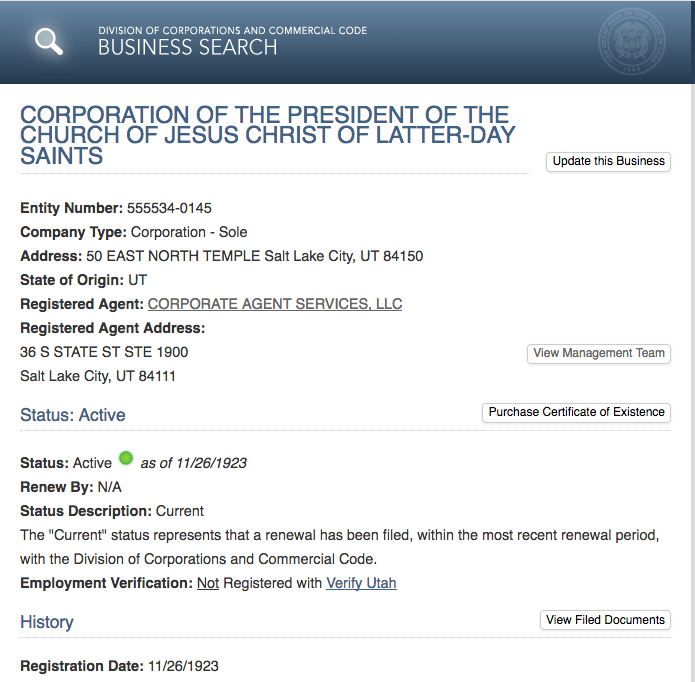
\includegraphics[width=1\linewidth]{articles/images/business.png}
  \caption{LDS Church Business Listing}
  \label{fig:business}
\end{figure}

Again, recently the church came out to declare that people shouldn't use the terms
``LDS" or ``Mormon" when speaking about the church. It should go by its full name.
``The Church of Jesus Christ of Latter-day Saints". Some people have gone to say that
by continuing to call yourself a Mormon, you are going against God's prophet and are
an apostate. With the constant use of the full church name, is that not saying
Christ's name too repeatedly?

According to scripture the Melchizedek Priesthood ``was called the Holy Priesthood, 
after the Order of the Son of God. But out of respect or reverence to the name of 
the Supreme Being, to avoid the too-frequent repetition of his name, 
they, the church, in the ancient days, called that priesthood after 
Melchizedek, or the Melchizedek Priesthood"\footnote{D\&C 107:3-4}

Is this not the same case? How can one be ``too-frequent repetition" and the other 
not?
\chapter{Nephi Kills Laben}

Question: When is it okay to kill another person?

Answer:

\begin{displayquote}
Thou shalt not kill.\footnote{Exodus 20:13}
\end{displayquote}

\begin{displayquote}
And again, the Lord God hath commanded that men should not 
murder.\footnote{2 Nephi 26:32}
\end{displayquote}

\begin{displayquote}
And now, behold, I speak unto the church. Thou shalt not kill; 
and he that kills shall not have forgiveness in this world, nor in the 
world to come.\footnote{D\&C 42:18}
\end{displayquote}

So, from the standard works, we have it that killing is bad. Murder is bad and evil
in the sight of God.

Yet, Nephi murdered Laben. Not only did he murder Laben, he hacked off his head.

If God can simply smite someone down\footnote{Abraham 1:20}, or cause a deep sleep 
to come upon them\footnote{Genesis 2:21}, why was it necessary for Nephi to kill 
Laben? He was ``constrained by the Spirit that [he] should kill 
Laban."\footnote{1 Nephi 4:10} Nephi admits he had never taken
another man's life. He resisted and resisted, and the spirit told Nephi ``Slay him,
for the Lord hath delivered him into thy hands."\footnote{1 Nephi 4:12}

So, Nephi chopped off Laben's head and went on his way. All because: ``It is better
that one man should perish than that a nation should dwindle and perish in
unbelief."\footnote{1 Nephi 4:13}
\chapter{Seer Stones}

Richard Bushman in Joseph Smith, Rough Stone Rolling explains:

\begin{displayquote}
Joseph had discovered two stones, one in 1822 while digging a well with Willard Chase 
a half mile from the Smith farm. (called the Chase seer stone) The source of the 
other stone is uncertain. These stones were the keys that enable Joseph to see 
things, as Lucy said, ``invisible to the natural eye." Emma Smith described one of 
them as ``a small stone, not exactly black, but was rather a dark color."

In 1841, Joseph showed his other, whitish stone to the Council of the Twelve in 
Nauvoo and told them, Brigham Young reported, ``that every man who lived on the 
earth was entitled to a seer stone and should have one, but they are kept from them 
in consequence of their wickedness."

Alva Hale...said Joseph Smith Jr. told him that the ``gift of seeing with a stone" 
was ``a gift from God" but that ``peeping" was all d\_\_d nonsense.\footnote{
Bushman, p. 48-52
} 
\end{displayquote}

We learn in D\&C 28, that a man by the name of Hiram Page claimed to have a seer
stone in his posession. But it was telling him things from the devil. So Satan has
power over seer stones. Yet, we are to believe that Joseph's seer stone never told
him anything from Satan?

\begin{displayquote}
And again, thou shalt take thy brother, Hiram Page, between him and thee alone, 
and tell him that those things which he hath written from that stone are not of me 
and that Satan deceiveth him;

For, behold, these things have not been appointed unto him, neither shall anything 
be appointed unto any of this church contrary to the church covenants.

For all things must be done in order, and by common consent in the church, by 
the prayer of faith.

And thou shalt assist to settle all these things, according to the covenants of 
the church, before thou shalt take thy journey among the Lamanites.

And it shall be given thee from the time thou shalt go, until the time thou shalt 
return, what thou shalt do.

And thou must open thy mouth at all times, declaring my gospel with the sound of 
rejoicing. Amen.\footnote{D\&C 28:11-16}
\end{displayquote}

We're also told that Joseph didn't need the seer stone when translating the bible
because he had learn the power of revelation since then. He didn't need an object
upon which to translate.

Seer Stones were used in magical thing like looking for money and hidden treasure in
Joseph's day. It doesn't seem to be something worthy of a prophet of God who had been
prepared since before the world was formed. It feels off and odd at times to think
about.
\chapter{Book of Mormon Translation}

For years members of the Church of Jesus Christ of Latter-day Saints were told that
Joseph Smith translated the Book of Mormon. It is said he translated it by the ``gift
and power of God." When people think of translation, they think he looked at the
plates and translated letter for letter, word for word the words of ancient prophets.

This was not the case. Joseph would place a seer stone in a hat, and put his face
into the hat. He would then read off the words as they appeared to him. The words on
the stone wouldn't change until his scribe confirmed back to him what was said.

The actual gold plates weren't used in the translation process at all.

People have brought up the question about how Bible passages, complete with changes
known to have been made by men, made it into the Book of Mormon. We have a possible
explaination for that. Joseph Smith copied the passages from the Bible into the 
Book of Mormon:

\begin{displayquote}
When Joseph Smith saw that the Nephite record was quoting the prophecies of Isaiah, 
of Malachi, and the words of the Savior, he took the English Bible and compared these 
passages as far as they paralleled each other, and finding that in substance in 
thought, they were alike, he adopted our English 
translation.\footnote{Young Men's Mutual Improvement Associations Manual, pp.
505-506, 1903-1904. New Witnesses for God. Volume II. The Book of Mormon Part I.
https://archive.org/stream/ymmia1903\#page/n699}
\end{displayquote}

So we're not even sure we have those passages copied word for word from the gold
plates. If that's the case? How are we to be sure that the rest of the book is really
the ``most correct book" out of them all?

There have been noted changes in the book throughout its history. The Eternal Father
being changed to Son of The Eternal Father for Christ etc. It seems to point towards
Joseph changing the words of the prophets. The idea of one god to three seperate
individuals.

But whenever someone questions the validity of the book, they are told to pray about
it. Taking Moroni's promise and seeing for themselves if it is true. Again, acting on
feelings alone and not evidence.

We were taught from the beginning, that the Book of Mormon is about the Native
Americans who came from Jerusalem. That is they were Jews. Science has determined
this not to be the case. The church had to make a change in the introduction of the
Book of Mormon, where it once said the Lamenite people ``are the principal ancestors 
of the American Indians", now it reads ``are among the ancestors of the American 
Indians."

If that change had to be made, what else about the book has been deemed wrong or
incorrect?

Some have come to believe that Joesph made the whole book up, that it was his
imagination which caused the Book of Mormon to come about. They claim the book is not
a historical document, but people should look on the principles taught within the
book which is more important than the origins.

The Book of Mormon stands as a keystone to the LDS Religion. If it is a fraud, then
the whole church is a fraud and Joseph Smith was not a prophet of God. Church leaders
have stated thusly, challenging those who would criticize the book.

The book itself states that if there are mistakes in it, those are the mistakes of
men (possibly the translation) and not of God.\footnote{Book of Mormon Title Page}

Why was the manner of translating the book never taught in a primary or sunday school
class? Why did it have to come out through other means? Those teachings were thought
to be anti-mormon lies and false doctrine, only to be proven later on they were true.
\chapter{Condemnation}

The Book of Mormon was pulbished in 1830. Exact date was 26 March 1830.\footnote{
Larry C. Porter, "From a Book Coming Forth," Ensign (July 1988), 42.} Though there
were parts of the book published in a newspaper in January of that same year.

However, 2 years later in September 1832 Joseph Smith received a revelation that the
church was under condemantion for forgetting the ``new covenant, even the Book of
Mormon." Two years? That seems pretty quick to place an entire church under
condemnation for not following scripture.

Here's the scripture in full:

\begin{displayquote}
And your minds in times past have been darkened because of unbelief, and because you 
have treated lightly the things you have received—

Which vanity and unbelief have brought the whole church under condemnation.

And this condemnation resteth upon the children of Zion, even all.

And they shall remain under this condemnation until they repent and remember the new 
covenant, even the Book of Mormon and the former commandments which I have given 
them, not only to say, but to do according to that which I have written.\footnote{
D\&C 84:54-57
}
\end{displayquote}
\chapter{A Volcano and a Family}

In 1815, the Tambora volcano erupted in Indonesia. It killed 80,000 people.\footnote{
https://www.history.com/this-day-in-history/volcanic-eruption-kills-80000
}

Because of this eruption the climate was affected worldwide, even to North America
where Joseph Smith Sr. and his family lived. With their crops ruined, they were
forced to move from Vermont to Palmyra New York. Five years after that Joseph Smith
had his First Vision.

These facts can be found in the new church history book titled ``Saints". It's in the
first chapter titled ``Ask in Faith".\footnote{https://history.lds.org/saints?lang=eng}

So let me get this straight. God kills over 80,000 people. Not just the people killed
in the volcano. Becuase of it, more than 80,000 people died due to starvation etc,
and Joseph Smith's family moved closer to the gold plates? So Joseph Sith Jr. could
find them? Couldn't have God found another way than killing over 80,000 of his
children? The narrative makes it sound like this was the cause for Joseph Smith Jr.
to be near the golden plates when the time came.

In the article ``A Year Without Summer"\footnote{
https://www.lds.org/ensign/1983/01/a-year-without-a-summer?lang=eng}, it simply
states that this volcano eruption ``played a small role in the history of The Church
of jesus Christ of Latter-day Saints."

I have a feeling God could have found other ways for Joseph Smith Sr. to move his
family instead of killing over 80,000 people.

It is interesting, a few chapter later in ``Saints", it speaks of Joseph trying to
get the gold plates. The angel warned him that if he had any evil thought in his mind
to use the plates to get gain, he could not obtain them.

When Joseph went to the hill to obtain the plates, upon seeing the other items in the
box which were valuable he placed the plates aside for a second. They disappeared.
The angel hid them from Joseph telling him he wasn't ready to take the plates.

If the angel could simply move them like that? Why was the volcano necessary?
\chapter{Law of Common Consent}

If a person doesn't support a policy that was given and is said to be revelation, how
exactly does that get handeled? I dare not ask, because there are a few policies
which I believe they are actually policies but not revelation.

Putting something in a handbook without telling the church is not revelation. That is
a policy change. The handbook is not scripture. Shouldn't revelation be considered
scripture? There is a line between scripture and that which is drafted by lawyers and
placed in a handbook. It even states it's a ``Policy".

\begin{displayquote}
Policies on Ordinances for Children of a Parent Living in a Same-Gender
Relationship\footnote{Changes to LDS Handbook 1- Document 2 Revised 11-3-2015.pdf}
\end{displayquote}

Since when has a policy become scripture or a revelation? Are not revelations from
the Lord considered scripture?\footnote{\textbf{Revelation:} Communication from God 
to His children on earth. Revelation may come through the Light of Christ and the 
Holy Ghost by way of inspiration, visions, dreams, or visits by angels. Revelation 
provides guidance that can lead the faithful to eternal salvation in the celestial 
kingdom.

The Lord reveals His work to His prophets and confirms to believers that the 
revelations to the prophets are true (Amos 3:7). Through revelation, the Lord 
provides individual guidance for every person who seeks it and who has faith, 
repents, and is obedient to the gospel of Jesus Christ. ``The Holy Ghost is a 
revelator," said Joseph Smith, and ``no man can receive the Holy Ghost without 
receiving revelations."

In the Lord’s Church, the First Presidency and the Quorum of the Twelve Apostles are 
prophets, seers, and revelators to the Church and to the world. The President of the 
Church is the only one whom the Lord has authorized to receive revelation for the 
Church (D\&C 28:2–7). Every person may receive personal revelation for his own 
benefit.

By every word that proceedeth out of the mouth of the Lord doth man live, Deut. 8:3
(Matt. 4:4; D\&C 98:11). [LDS.org]}

So, what becomes of it all? If things in the handbook are considered revelation, but
not scripture. It becomes confusing, and goes against the law of common consent. The
law of common consent is stated as follows:

\begin{displayquote}
Not only are Church officers sustained by common consent, but this same principle 
operates for policies, major decisions, acceptance of new scripture, and other things 
that affect the lives of the Saints (see D\&C 26:2).\footnote{``Section 26, The Law 
of Common Consent," Doctrine and Covenants Student Manual (2002), 54}
\end{displayquote}

As far as I am aware, there hasn't been a sustaining vote on a revelation since the
1978 announcement of the ban on the blacks in General Conference.\footnote{
``Revelation on Priesthood Accepted, Church Officers Sustained," October 1978 General
Conference, LDS.org
}

It would be interesting to list policies and revelations which haven't been voted on,
I'll start with the most recent and work my way backwards? Maybe? Who knows how far I
can go with it. These have been stated as being revelation.

\begin{enumerate}
\item No longer referring to the church as the Mormon church (2018)
\item Discontinuing Home Teaching, adopting Ministering (2018)
\item Combining Elders Quorum and High Priests Group into one Elders Quroum (2018)
\item Children of Same-Gender Relationships (2015)
\item Lowering of Mission Ages (2012)
\end{enumerate}

I heard it considered that because a group sustains the prophet, they don't have to
live by the law of common consent. That because they sustain the prophet, they
automatically accept whatever revelation that comes and is announced. (For the
  record, the Children of Same-Gender Relationships policy, wasn't revealed to
  the membership of the church until after it was leaked. It was snuck in Handbook
  1.)

Then Apostle Russel M. Nelson had the following to say regarding the policy:

\begin{displayquote}
We sustain 15 men who are ordained as prophets, seers, and revelators. When a thorny 
problem arises-and they only seem to get thornier each day-these 15 men wrestle with 
the issue, trying to see all the ramifications of various courses of action, and they 
diligently seek to hear the voice of the Lord. After fasting, praying, studying, 
pondering, and counseling with my Brethren about weighty matters, it is not unusual 
for me to be awakened during the night with further impressions about issues with 
which we are concerned. And my Brethren have the same experience.

The First Presidency and Quorum of the Twelve Apostles counsel together and share 
all the Lord has directed us to understand and to feel individually and collectively. 
And then we watch the Lord move upon the President of the Church to proclaim the 
Lord's will.

This prophetic process was followed in 2012 with the change in minimum age for 
missionaries and again with the recent additions to the Church's handbook, 
consequent to the legalization of same-sex marriage in some countries. Filled with 
compassion for all, and especially for the children, we wrestled at length to 
understand the Lord’s will in this matter. Ever mindful of God's plan of salvation 
and of His hope for eternal life for each of His children, we considered countless 
permutations and combinations of possible scenarios that could arise. We met 
repeatedly in the temple in fasting and prayer and sought further direction and 
inspiration. And then, when the Lord inspired His prophet, President Thomas S. 
Monson, to declare the mind of the Lord and the will of the Lord, each of us during 
that sacred moment felt a spiritual confirmation. It was our privilege as Apostles 
to sustain what had been revealed to President Monson. Revelation from the Lord to 
His servants is a sacred process, and so is your privilege of receiving personal 
revelation.\footnote{Becoming True Millennials, Russel M. Nelson, January 10, 2016 
Devotional}
\end{displayquote}

\chapter{Apostasy}

According to the Church's website, Apostasy is ``when individuals or groups of people
turn away from the principles of the gospel."\footnote{Apostasy, LDS.org}

When a person is in apostasy, they are requried to undergo a Church Disciplinary
Council. There are guidelines when such a council is mandatory. It also defines
Apostasy:

\begin{displayquote}
\textbf{Apostasy}\footnote{Handbook 1, 6.7.3}

As used here, \textit{apostasy} refers to members who:

\begin{enumerate}
\item Repeatedly act in clear, open, and deliberate public opposition to the Church 
  or its leaders.

\item Persist in teaching as Church doctrine information that is not Church doctrine 
  after they have been corrected by their bishop or a higher authority.

\item Continue to follow the teachings of apostate sects (such as those that advocate 
  plural marriage) after being corrected by their bishop or a higher authority.

\item Are in a same-gender marriage.

\item Formally join another church and advocate its teachings.
\end{enumerate}
\end{displayquote}
\chapter{Excommunication}

When someone goes against the church's teachings and openly oppose the church and its
leaders, they can be excommunicated from the LDS Church. Figure \ref{fig:ex1} is an 
example of such:

\begin{figure}[h!]
  \centering
  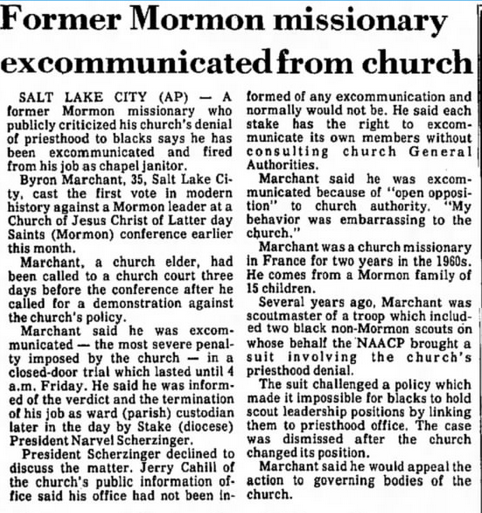
\includegraphics[width=0.4\linewidth]{articles/images/ex.png}
  \caption{The Daily Reporter (Dover, Ohio) 15 Oct 1977}
  \label{fig:ex1}
\end{figure}

In the early days of the church, leaders were known to excommunicate followers more
often and loose. It has slowed down a bit as church goers have gotten in line as it
were. But there are still excommunications which happen every year. Of course, not 
all end up in the newspaper like Figure \ref{fig:ex1}. But it still happens.

It was said during the succession crisis of 1844 after Joseph Smith died, anyone who
voted against Brigham Young were excommunicated. Even though a vote for and against
was called for. Anytime a person in the church votes against or opposing the leadders
of the church, they are in danger of apostasy.

To face excommunication from the church, you are taken off the roles of the church.
Your baptism becomes null and void, any temple blessings are revoked. You are not
able to speak in a church meeting, give a prayer, take the sacrament or participate
in any way at all.

Some people are shunned by their family members. This is not a church teaching to be
shunned, but it does happen. Family can't accept that one would not want to follow a
church they grew up in. They cannot understand how a person would abandon their God
as it were.

I think that's a main issue poeple don't understand. Just because a person is
excommunicated from the church, it doesn't mean they have lost faith in Christ and a
belief in God. Perhaps they have come to understand Christ a little bit more than
they did when in the LDS faith.

The leaders say it's to help the repentence process, to help others come back to the
church and to accept Christ's atonement in their lives. In effect, the church will
not leave them alone. If a person is openly opposing church leaders, maybe they want
to be left alone. It's a thought.

Members ask all the time to be left alone from the church, yet because the member is
on the role the church continues to visit the member. The only way to avoid any of
this is to either be excommunicated or to request your name be removed from the
records of the church.

Even removing your name isn't an easy process. The bishop of the local ward will
still want to see if there's anything they can do to help you come back to the fold.
It's a never ending process which constantly loops over again.

It's sad to think about.

In a talk given to the All-Church Coordinating Council, Boyd K. Packer said the
following:

\begin{displayquote}
There are three areas where members of the Church, influenced by social and political 
unrest, are being caught up and led away. I chose these three because they have made 
major invasions into the membership of the Church. In each, the temptation is for us 
to turn about and face the wrong way, and it is hard to resist, for doing it seems 
so reasonable and right.

The dangers I speak of come from the gay-lesbian movement, the feminist movement 
(both of which are relatively new), and the ever-present challenge from the so-called 
scholars or intellectuals.\footnote{Talk to the All-Church Coordinating Council,
Elder Boyd K. Packer, May 18, 1993}
\end{displayquote}

If a person in the church identifies with any of these three, they can face church
discipline. That may come in the form of excommunication, or the lesser judgement of
disfellowship.

To openly think for yourself goes against church teachings. You are to obey the
commandments the church has laid out, which they claim come from the Lord. Only then
will you be able to be in full fellowship with the Church of Chirst. Any deviation
from this path and you are facing dangerous waters.

In the same breath LDS faithful are taught to seek out learning and to seek things
which are good. They are taught to seek if something is right or not. To not blindly
follow a prophet of God but to learn for themselves if the teachings are true. Once
they learn if it is true or false they can come to a decision.

But if you decided what a prophet of God has spoken to be false, you are on thin ice
and there is no real coming back from that. The official statment is the church must
protect its good name.\footnote{
The purposes of disciplinary councils are to save the souls of transgressors, 
protect the innocent, and safeguard the purity, integrity, 
and good name of the Church.
https://www.lds.org/topics/church-disciplinary-councils?lang=eng
}

So, does that mean forget about the people who are trying to learn from the best
books and who might bring about history issues? Who are simply trying to understand
the religion they have believed in their whole life? There's a lot to be said about
the church's history, not all is good mind you. There is a lot to be said about all
of it. Choosing what you want to believe to be true and what is true? That's not how
any of this works.

Jesus cared more about the people then he did protecting a church. Even when Saul was
persecuting the church, Jesus appeared to him (it still isn't clear which way Jesus
appeared to Saul, be it visual or audio\footnote{Acts 9:7; Acts 22:9}), 
and Saul changed his ways. Jesus was concerned about Saul and the people, the people 
Saul was persecuting. Jesus didn't care about the ``good name of the church", He 
cared about the people.
\chapter{Quotes}

\begin{displayquote}
Say nothing of my religion. It is known to my God and myself alone. Its evidence 
before the world is to be sought in my life; if that has been honest and dutiful 
to society, the religion which has regulated it cannot be a bad one.\footnote{
Thomas Jefferson
}
\end{displayquote}

Quotes abound in the world of religion. There are so many religious quotes out 
there, some days I do not know where some begin and others end. They are that 
which bring forth the breath of life into people. Allowing them to try and see 
all that is out there.

Granted, not all quotes are faith promoting. There are quotes out there which 
people would rather be buried never to see the light of day. But still those 
quotes exist for a reason. Sometimes those reasons are more than we can grasp 
at the current moment in time.

\begin{displayquote}
If we have the truth, it cannot be harmed by investigation. 
If we have not the truth, it ought to be harmed.\footnote{
President J. Reuben Clark}
\end{displayquote}

The truth is out there. One just has to want to look for it. It isn't hiding. 
In most instances the truth is there, in plain sight. If we do not actually 
look for the truth or seek it out, we cannot find the truth. It will seldom 
come to find us.

\begin{displayquote}
The man who cannot listen to an argument which opposes his views either has a 
weak position or is a weak defender of it. No opinion that cannot stand 
discussion or criticism is worth holding. And it has been wisely said that 
the man who knows only half of any question is worse off than the man who 
knows nothing of it. He is not only one sided, but his partisanship soon 
turns him into an intolerant and a fanatic. In general it is true that nothing 
which cannot stand up under discussion and criticism is worth
defending.\footnote{James E. Talmage}
\end{displayquote}

\begin{displayquote}
We desire that the brethren and sisters will all feel the responsibility of 
expressing their feelings in relation to the propositions that may be put 
before you. We do not want any man or woman who is a member of the Church to 
violate their conscience. We would like all to vote as they feel, whether for 
or against.\footnote{President Joseph F. Smith}
\end{displayquote}

Men and Women are free to choose according to their own thoughts. That is the 
will and mind of the Lord. For we were all given agency th at we might choose 
good from evil. Without having such a choice, we wouldn't learn or grow from 
that which comes across our path in this life.

There are other quotes by church leaders which are not quite in tune with that 
which we have today. Some quotes have been disavowed, others have been simply 
said the person speaking was saying such things as a man.

\begin{displayquote}
Live a good life. If there are gods and they are just, then they will not care 
how devout you have been, but will welcome you based on the virtues you have 
lived by. If there are gods, but unjust, then you should not want to worship 
them. If there are no gods, then you will be gone, but will have lived a noble 
life that will live on in the memories of your loved ones.\footnote{
Marcus Aurelius}
\end{displayquote}

Isn't that what this life is all about? Living a good life? Shouldn't that be
what this life is all about? Do unto others as you would have them do unto you?
Come on now, it can't be this difficult.

\begin{displayquote}
Cherish your doubts, for doubt is the attendant of truth. Doubt is the key to the
door of knowledge; it is the servant of discovery. A belief which may not be
questioned binds us to error, for there is incompleteness and imperfection in every
belief. Doubt is the touchstone of truth; it is an acid which eats away the false.
Let no one fear the truth, that doubt may consume it; for doubt is a testing of
belief. The truth stands boldly and unafraid; it is not shaken by the testing:
For truth, if it be truth, arises from each testing stronger, more secure. Those
that would silence doubt are filled with fear; their houses are built on shifting
sands. But those who fear not doubt, and know its use, are founded on rock.
They shall walk in the light of growing knowledge; the work of their hands shall
endure. Therefore let us not fear doubt, but let us rejoice in its help: It is to be
the wise as a staff to the blind; doubt is the attendant of truth.\footnote{
Robert T. Weston}
\end{displayquote}

The LDS (Mormon) Church has an issue of anti-intelectualism. See the following:

\begin{displayquote}
He [Satan] wins a great victory when he can get members of the church to speak
against their leaders and to do their own thinking. When our leaders speak, the
thinking has been done. When they propose a plan – it is God's Plan. When they point
the way, there is no other which is safe. When they give directions, it should mark
the end of controversy, God works in no other way. To think otherwise, without 
immediate repentance, may cost one his faith, may destroy his testimony, and leave 
him a stranger to the Kingdom of God.\footnote{
Ward Teacher's Message, Deseret News, Church Section, p. 5, May 26, 1945; see also 
Improvement Era, June 1945
}
\end{displayquote}

\begin{displayquote}
Always keep your eye on the President of the church, and if he ever tells you to do
anything, even if it is wrong, and you do it, the lord will bless you for it, but you
don't need to worry. The lord will never let his mouthpiece lead the people
astray.\footnote{Apostle Marion G. Romney, Conference Report, Oct. 1960, p. 78}
\end{displayquote}

\begin{displayquote}
When Elder Packer interviewed me as a prospective member of Brigham Young
University's faculty in 1976, he explained: ``I have a hard time with historians
because they idolize the truth. The truth is not uplifting; it destroys. I could tell
most of the secretaries in the church office building because that they are ugly and
fat. That would be the truth, but it would hurt and destroy them. Historians should
tell only that part of the truth that is inspiring and uplifting."\footnote{
D. Michael Quinn, “On Being a Mormon Historian (and Its Aftermath),” in George D. 
Smith, ed., Faithful History: Essays on Writing Mormon History, 1992, p. 76
}
\end{displayquote}

\begin{displayquote}
When the Prophet speaks the debate is over.\footnote{Apostle N. Eldon Tanner, 
Ensign, Aug. 1979, pp. 2-3.}
\end{displayquote}

\begin{displayquote}
Avoid those who would tear down your faith. Faith-killers are to be shunned. The
seeds which they plant in the minds and hearts of men grow like cancer and eat
away the Spirit.\footnote{Carlos E. Asay, October 1981 General Conference}
\end{displayquote}

\begin{displayquote}
No true Latter-day Saint will ever take a stand that is in opposition to what the 
Lord has revealed to those who direct the affairs of his earthly kingdom. No 
Latter-day Saint who is true and faithful in all things will ever pursue a course, 
or espouse a cause, or publish an article or book that weakens or destroys 
faith.\footnote{Apostle Bruce R. McConkie, October 1984 General Conference}
\end{displayquote}

\begin{displayquote}
Some things that are true are not edifying or appropriate to communicate. Readers 
of history and biography should ponder that moral reality as part of their effort to 
understand the significance of what they read.\footnote{Apostle Dallin H. Oaks, 
``Reading Church History," Ninth Annual Church Educational System Religious 
Educators' Symposium, August 16, 1985, Brigham Young University}
\end{displayquote}

\begin{displayquote}
There are three areas where members of the Church, influenced by social and political
unrest, are being caught up and led away. I chose these three because they have made
major invasions into the membership of the Church. In each, the temptation is for us
to turn about and face the wrong way, and it is hard to resist, for doing it seems
reasonable and right.

The dangers I speak of come from the gay-lesbian movement, the feminist movement
(both of which are relatively new), and the ever-present challenge from the so-called
scholars or intellectuals. Our local leaders must deal with all three of them with
ever increasingly frequency. In each case, the members who are hurting have the
conviction that the Church somehow is doing something wrong to members or that the
Church is not doing enough for them.\footnote{Apostle Boyd K. Packer, 
``Talk to the All-Church Coordinating Council," May 18, 1993}
\end{displayquote}

\begin{displayquote}
The Church warns its members against symposia and similar gatherings that include
presentations that (1) disparage, ridicule, make light of, or are otherwise
inappropriate in their treatment of sacred matters or (2) could injure the Church,
detract from its mission, or jeopardize its members’ well-being. Members should not
allow their position or standing in the Church to be used to promote or imply
endorsement of such gatherings.\footnote{Section 17.1.46 of Handbook 1 for Stake 
Presidents and Bishops.}
\end{displayquote}

\begin{displayquote}
Doubt your doubts before you doubt your faith.\footnote{Dieter F. Uchtdorf, 
October 2013 General Conference}
\end{displayquote}

\begin{displayquote}
Another claim we sometimes hear is that the leaders won’t answer our doubts. Doubts.
Here we need to define the difference between doubts and questions. Questions, when
asked with a sincere desire to increase ones understanding and faith, are again
encouraged. Such questions, questions we call them, are asked with the real intent of
better understanding and more fully obeying the will of the Lord. Questions are very
different from doubts. ... One difference between questions asked in faith and doubts
is that questions lead to faith and to revelation whereas doubts lead to
disobedience, which in turn renders people less able to receive revelation, or in
other words, doubt is darkness. Questions asked in faith lead to light.\footnote{
Apostle Dallin H. Oaks and Assistant Church Historian Richard E. Turley Jr. 
during the Boise Rescue on June 13th, 2015.
}
\end{displayquote}

\begin{displayquote}
Some who use personal reasoning or wisdom to resist prophetic direction give
themselves a label borrowed from elected bodies -- ``the loyal opposition." However
appropriate for a democracy, there is no warrant for this concept in the government
of God’s kingdom, where questions are honored but opposition is not.\footnote{
Apostle Dallin H. Oaks, April 2016 General Conference
}
\end{displayquote}

The church doesn't like people researching its history. Why is that exactly? What
does it have to hide that's so bad, it's afraid of letting people know its full
history?
\chapter{My Creed}
\begin{enumerate}
\item It is a noble thing to be doing that which is good. 
The works of men who do follow the God who gave them life is good 
and honorable.

\item We know of God and His ways and of His son Jesus Christ.

\item Jesus Christ came into the world to take upon Him the sins of the world.

\item  That same Jesus was born of a mortal mother and an immortal father, 
allowing Him the power over death to come forth in resurrection.

\item We believe of the Holy Spirit also known as the Holy Ghost who is 
able to dwell in the hearts of men as a testimony of God the Eternal Father 
and His Son, Jesus Christ.

\item We believe the Eternal Father, Jesus Christ, and the Holy Ghost to be of 
one purpose but not one body, for they are three separate distinct individuals. 
The Father and The Son having bodies of flesh and bone, for they have been 
resurrected, and the Holy Ghost to be a personage of spirit.

\item We sustain the doctrine that man may be saved through the redemption 
which Christ laid out for the world, that redemption being an eternal sacrifice, 
a final sacrifice to fulfill the law.

\item And to this end was Christ crucified that we might be saved in the 
kingdom of our Father.

\item We affirm in the coming days that we will come before God to be 
judged according to our works, thus being saved by the grace of Christ.

\item We believe these things to be true, even so Amen.
\end{enumerate}

\newpage

\appendix
\section{Appendix A: Lilith}

With all of the possible changes in the narrative throughout the years, there is
mention of a woman named Lilith. She was supposed to be Adam's first wife. But
she didn't want to follow what he said and she ran.

I include it here for a twofold purpose.

1. Do we know this isn't true for certain? It could have been removed from the
texts of the bible for all we know.

2. There is some confusion regarding Genesis 1:27 where it stats that God
created male and female. Then in the next chapter he creates them again.

Some have said there are two versions of the creation. Some have tried to state
(falsely based on the book of Moses) that this was the pre-existence creation of
Adam and Eve.

The pre existence had already been created.

The follow text is quoted from Hebrew Myths\cite{myth}:

Chapter 10: Adam's Helpmeets

(a) Having decided to give Adam a helpmeet lest he should be alone
of his kind, God put him into a deep sleep, removed one of his
ribs, formed it into a woman, and closed up the wound, Adam awoke
and said: `This being shall be named ``Woman", because she has been
taken out o f man. A man and a woman shall be one flesh.' The
title he gave her was Eve, `the Mother of 
All Living''.\footnote{Genesis II. 18-25; III. 20.}

(b) Some say that God created man and woman in His own image on
the Sixth Day, giving them charge over the 
world;\footnote{Genesis I. 26-28.} but that Eve
did not yet exist. Now, God had set Adam to name every beast, bird
and other living thing. When they passed before him in pairs, male
and female, Adam-being already like a twenty-year-old man-felt
jealous of their loves, and though he tried coupling with each
female in turn, found no satisfaction in the act. He therefore
cried: `Every creature but I has a proper matel', and prayed God
would remedy this injustice.\footnote{Gen. Rab. 17.4; B. Yebamot 632.}

(c) God then formed Lilith, the first woman, just as He had
formed Adam, except that He used filth and sediment instead of
pure dust. From Adam's union with this demoness, and with another
like her named Naamah, Tubal Cain's sister, sprang Asmodeus and
innumerable demons that still plague mankind. Many generations
later, Lilith and Naamah came to Solomon's judgement seat,
disguised as harlots of 
Jerusalem'.\footnote{Yalqut Reubeni ad. Gen. II. 21; IV. 8.}

(d) Adam and Lilith never found peace together; for when he
wished to lie with her, she took offence at the recumbent posture
he demanded. `Why must I lie beneath you?' she asked. `I also was
made from dust, and am therefore your equal.' Because Adam tried
to compel her obedience by force, Lilith, in a rage, uttered the
magic name of God, rose into the air and left him.

Adam complained to God: `I have been deserted by my helpmeet' God
at once sent the angels Senoy, Sansenoy and Semangelof to fetch
Lilith back. They found her beside the Red Sea, a region abounding
in lascivious demons, to whom she bore lilim at the rate of more
than one hundred a day. `Return to Adam without delay,' the angels
said, `or we will drown you!' Lilith asked: `How can I return to
Adam and live like an honest housewife, after my stay beside the
Red Sea?? `It will be death to refuse!' they answered. `How can I
die,' Lilith asked again, `when God has ordered me to take charge
of all newborn children: boys up to the eighth day of life, that
of circumcision; girls up to the twentieth day. None the less, if
ever I see your three names or likenesses displayed in an amulet
above a newborn child, I promise to spare it.' To this they
agreed; but God punished Lilith by making one hundred of her demon
children perish 
daily;\footnote{Alpha Beta diBen Sira, 47; Gaster, MGWJ, 29 (1880), 553 ff.}
and if she could not destroy a human
infant, because of the angelic amulet, she would spitefully turn
against her own.\footnote{Num. Rab. 16.25.}

(e) Some say that Lilith ruled as queen in Zmargad, and again in
Sheba; and was the demoness who destroyed job's 
sons.\footnote{Targum ad job 1. 15.} Yet she escaped the curse of death which 
overtook Adam, since they had parted long before the Fall. Lilith and 
Naamah not only strangle infants but also seduce dreaming men, any one of 
whom, sleeping alone, may become their 
victim.\footnote{B. Shabbat 151b; Ginzberg, LJ, V. 147-48.}

(f) Undismayed by His failure to give Adam a suitable helpmeet,
God tried again, and let him watch while he built up a woman's
anatomy: using bones, tissues, muscles, blood and glandular
secretions, then covering the whole with skin and adding tufts of
hair in places. The sight caused Adam such disgust that even when
this woman, the First Eve, stood there in her full beauty, he felt
an invincible repugnance. God knew that He had failed once more,
and took the First Eve away. Where she went, nobody knows for
certain.\footnote{Gen. Rab. 158, 163-64; Mid. Abkir 133, 135; 
Abot diR. Nathan 24; B. Sanhedrin 39a.}

(g) God tried a third time, and acted more circumspectly. Having
taken a rib from Adam's side in his sleep, He formed it into a
woman; then plaited her hair and adorned her, like a bride, with
twenty-four pieces of jewellery, before waking him. Adam was
entranced.\footnote{Gen. II. 21-22; Gen. Rab. 161.}

(h) Some say that God created Eve not from Adam's rib, but from a
tail ending in a sting which had been part of his body. God cut
this off, and the stump-now a useless coccyx-is still carried by
Adam's descendants.\footnote{Gen. Rab. 134; B. Erubin 18a.}

(i) Others say that God's original thought had been to create two
human beings, male and female; but instead He designed a single
one with a male face looking forward, and a female face looking
back. Again He changed His mind, removed Adam's backward-looking
face, and built a woman's body for it.\footnote{B. Erubin 18a.}

 (j) Still others hold that Adam was originally created as an
androgyne of male and female bodies joined back to back. Since
this posture made locomotion difficult, and conversation awkward,
God divided the androgyne and gave each half a new rear. These
separate beings He placed in Eden, forbidding them to 
couple.\footnote{Gen. Rab. 55; Lev. Rab. 14.1: Abot diR. Nathan 1.8; B.
Berakhot 61a; B. Erubin 18a; Tanhuma Tazri'a 1; Yalchut Gen. 20;
Tanh. Buber iii.33; Mid. Tehillim 139, 529.}

There is no way of knowing if these thoughts are true or if they are of fable.
The truth will eventually come forth in time naturally, but with all of the
changes of the Bible that have taken place, who is to know for sure exactly if
what is in the Bible can be taken as truth.

Either way, this is an interesting insight into human thought on the matter.
Changes come and go, there will always be changes it would seem.
\chapter{J. Reuben Clark: The Church Years}

By 1917, however, Reuben was asking himself some religious questions that took 
him years to resolve. In one personal memo he began, ``If we have truth, [it] 
cannot be harmed by investigation. If we have not truth, it ought to be harmed." 
From that premise he added the observation that scientists and lawyers 
(like himself) were not blindly believing and that they must refuse to be 
deceived by others or by their own wishful thinking. ``A lawyer must get at 
facts, he must consider motives -- he must tear off the mask and lay bare the 
countenance, however hideous. The frightful skeleton of truth must always be 
exposed ... [the lawyer] must make every conclusion pass the fiery ordeal of 
pitiless reason. If their conclusions cannot stand this test, they are false." 
During the same year the increasingly introspective lawyer asked himself the 
questions: Are we not only entitled, but expected to think for ourselves? 
Otherwise where does our free agency come in? His answer was a resounding: 
``If we are blindly to follow some one else we are not free agents.... 
That we may as a Church determine for ourselves our course of action, is 
shown by the Manifesto [abandoning the practice of polygamy]. We may not 
probably take an affirmative stand, i.e., adopt something new but we may 
dispense with something." Perhaps he had never before questioned the assumptions 
that lay behind some of the simple faith of his youth, but at midlife J. 
Reuben Clark, Jr. proclaimed that there must be no forbidden questions in 
Mormonism.

The directions to which his philosophy of religious inquiry led him were 
indicated in his musings about two essentials of Mormonism: the revelations of 
Joseph Smith, Jr. and the Church belief in progression toward godhood. As he 
examined the revelations in the Doctrine and Covenants concerning the structure 
of the Church government, Reuben Clark wondered to what extent Joseph Smith's 
reading or experience, ``his own consciousness," had contributed to what he set 
down, and when Reuben pondered the Mormon belief in the potential of individuals 
to attain the godly stature of their Father in Heaven, his logical mind boggled 
a bit. ``Is Space or occupied portions of it divided among various deities -- 
have they great `spheres of influence'? War of Gods -- think of wreck of matter 
involved -- if matter used -- or would it be a war of forces?" In his 
mid-forties, he regarded these as legitimate doctrinal inquiries but soon 
realized that each question concerning doctrine led to other questions, each 
of which was further removed from rational verification. Reuben soon came to the 
conclusion he described in later years to the non-Mormon president of George 
Washington University: ``For my own part I early came to recognize that for me 
personally I must either quit rationalizing ... or I must follow the line of 
my own thinking which would lead me I know not where."

But J. Reuben Clark soon recognized where an uncompromising commitment to 
rational theology would lead him, and he shrank from the abyss. 
``I came early to appreciate that I could not rationalize a religion for myself, 
and that to attempt to do so would destroy my faith in God," 
he later wrote to his non-Mormon friend. ``I have always rather worshipped 
facts," he continues,``and while I thought and read for a while, many of the 
incidents of life, experiences and circumstances led, unaided by the spirit of 
faith, to the position of the atheist, yet the faith of my fathers led me to 
abandon all that and to refrain from following it.... For me there seemed to be 
no alternative. I could only build up a doubt. --If I were to attempt to 
rationalize about my life here, and the life too come, I would be drowned in 
a sea of doubt."

All the confidence of J. Reuben Clark's commitment to rational inquiry in 
religious matters evaporated. He had once believed that in intellectual faith 
``we may not probably take an affirmative stand, i.e., adopt something new but 
we may dispense with something," but Reuben found that such an attempt could 
only lead to dispensing with everyting [sic]. As he cast about for some way of 
explaining his position to others, he discovered an anecdote about Abraham 
Lincoln, who justified reading the Bible despite his reputed agnosticism with 
the comment: ``I have learned to read the Bible. I believe all I can and take 
the rest on faith." To a friend, Reuben related the Lincoln story and added, 
``Substituting in the substance the words `our Mormon Scriptures,' you will 
have about my situation." He later commended that anecdote to a general 
conference of the Church. Convinced that no religious faith could withstand 
uncompromising intellectual inquiry, Reuben concluded that in Babylon as well 
as in Zion, the refusal to rationalize one's religious beliefs was the highest 
manifestation of faith.

\cite{clark}
\chapter{An Address to All Believers in Christ}

Joseph looked into the hat in which he placed the stone, and received a 
revelation that some of the brethren should go to Toronto, Canada, and that 
they would sell the copyright of the Book of Mormon. Hiram Page and Oliver 
Cowdery went to Toronto on this mission, but they failed entirely to sell the 
copyright, returning without any money. Joseph was at my father's house when 
they returned. I was there also, and am an eye witness to these facts. Jacob 
Whitmer and John Whitmer were also present when Hiram Page and Oliver Cowdery 
returned from Canada. Well, we were all in great trouble; and we asked Joseph 
how it was that he had received a revelation from the Lord for some brethren to 
go to Toronto and sell the copyright, and the brethren had utterly failed in 
their undertaking. Joseph did not know how it was, so he enquired of the Lord 
about it, and behold the following revelation came through the stone: 
`Some revelations are of God: some revelations are of men: and some 
revelations are of the devil.' So we see that the revelation to go to 
Toronto and sell the copyright was not of God, but was of the devil 
or of the heart of man.

\cite{whitmer}
\chapter{ON MARRIAGE}

According to the custom of all civilized nations, marriage is regulated by laws and
ceremonies: therefore we believe, that all marriages in this church of Christ of
Latter Day Saints, should be solemnized in a public meeting, or feast, prepared for
that purpose: and that the solemnization should be performed by a presiding high
priest, high priest, bishop, elder, or priest, not even prohibiting those persons who
are desirous to get married, of being married by other authority.-We believe that it
is not right to prohibit members of this church from marrying out of the church, if
it be their determination so to do, but such persons will be considered weak in the
faith of our Lord and Savior Jesus Christ.

Marriage should be celebrated with prayer and thanksgiving; and at the solemnization,
the persons to be married, standing together, the man on the right, and the woman on
the left, shall be addressed, by the person officiating, as he shall be directed by
the holy Spirit; and if there be no legal objections, he shall say, calling each by
their names: ``You both mutually agree to be each other's companion, husband and wife,
observing the legal rights belonging to this condition; that is, keeping yourselves
wholly for each other, and from all others, during your lives." And when they have
answered ``Yes," he shall pronounce them ``husband and wife" in the name of the Lord
Jesus Christ, and by virtue of the laws of the country and authority vested in him:
``may God add his blessings and keep you to fulfil [fulfill] your covenants from
henceforth and forever. Amen."

The clerk of every church should keep a record of all marriages, solemnized in his 
branch.

All legal contracts of marriage made before a person is baptized into this church,
should be held sacred and fulfilled. Inasmuch as this church of Christ has been
reproached with the crime of fornication, and polygamy: we declare that we believe,
that one man should have one wife; and one woman, but one husband, except in case of
death, when either is at liberty to marry again. It is not right to persuade a woman
to be baptized contrary to the will of her husband, neither is it lawful to influence
her to leave her husband. All children are bound by law to obey their parents; and to
influence them to embrace any religious faith, or be baptized, or leave their parents
without their consent, is unlawful and unjust. We believe that husbands, parents and
masters who exercise control over their wives, children, and servants and prevent
them from embracing the truth, will have to answer for that sin.

We have given the above rule of marriage as the only one practiced in this church, to
show that Dr. J. C. Bennett's ``secret wife system" is a matter of his own
manufacture; and further to disabuse the public ear, and shew [show] that the said
Bennett and his misanthropic friend Origen Bachelor, are perpetrating a foul and
infamous slander upon an innocent people, and need but be known to be hated and
despise. In support of this position, we present the following certificates:-

We the undersigned members of the church of Jesus Christ of Latter-Day Saints and
residents of the city of Nauvoo, persons of families do hereby certify and declare
that we know of no other rule or system of marriage than the one published from the
Book of Doctrine and Covenants, and we give this certificate to show that Dr. J. C.
Bennett's ``secret wife system"

(page 939)

is a creature of his own make as we know of no such society in this place nor never 
did.

S. Bennett, N. K. Whitney,

George Miller, Albert Pettey,

Alpheus Cutler, Elias Higbee,

Reynolds Cahoon, John Taylor,

Wilson Law, E. Robinson,

W. Woodruff, Aaron Johnson.

We the undersigned members of the ladies' relief society, and married females do
certify and declare that we know of no system of marriage being practised [practiced]
in the church of Jesus Christ of Latter Day Saints save the one contained in the Book
of Doctrine and Covenants, and we give this certificate to the public to show that J.
C. Bennett's ``secret wife system" is a disclosure of his own make.

Emma Smith, President,

Elizabeth Ann Whitney, Counsellor [Counselor],

Sarah M. Cleveland, Counsellor [Counselor],

Eliza R. Snow, Secretary,

Mary C. Miller, Catharine Pettey,

Lois Cutler, Sarah Higbee,

Thirza Cahoon, Phebe Woodruff

Ann Hunter, Leonora Taylor,

Jane Law, Sarah Hillman,

Sophia R. Marks, Rosannah Marks,

Polly Z. Johnson, Angeline Robinson,

Abigail Works.

(Times and Seasons Vol 3 No 23)

\backmatter
\printbibliography

\end{document}